\documentclass[a4paper,12pt]{article}
\usepackage{docsTemplate}
\usepackage{longtable}
\usepackage{float}
\usepackage[official]{eurosym}
\usepackage{pgf-pie}
\usepackage{makecell}
\usepackage{xltabular}
\usepackage{amsmath}

\usepackage{titlesec}
\setlength{\headheight}{23.3111pt}

\titleformat{\paragraph}[block]
  {\normalfont\normalsize\bfseries}
  {\theparagraph}{1em}{}

\titlespacing*{\paragraph}{0pt}{3.25ex plus 1ex minus .2ex}{1.5ex}

\setTitle{Piano di Progetto}
\setAuthors{Bianca Zaghetto \\ & Mattia Oliva Medin \\ & Sara Gioia Fichera \\ & Nenad Radulovic \\ & Filippo Compagno \\ & Andrea Masiero \\ & Francesco Balestro}
\setVerificators{Mattia Oliva
Medin \\ & Sara Gioia
Fichera \\ & Andrea Masiero \\ & Nenad Radulovic \\ & Filippo
Compagno \\ & Francesco Balestro \\ & Bianca Zaghetto}
\setApprovation{Nenad Radulovic}
\setVersion{1.5}
\setType{Esterno}
\setDestination{Tullio Vardanega \\ & Riccardo Cardin \\ & Sanmarco Informatica \\[-0.1em] & Team Three Technologies}
\setcounter{secnumdepth}{4}
\setcounter{tocdepth}{4}

\begin{document}
\include{docTitlepage}

\newpage
\section*{Registro delle modifiche}
\rowcolors{2}{lightgray}{white}
\begin{xltabular}{\textwidth}{|l|l|X|l|X|X|}
\hline
\textbf{Vers.} & \textbf{Data} & \textbf{Autore} & \textbf{Ruolo} & \textbf{Verifica} & \textbf{Oggetto} \\
\hline
\endhead
\endfoot
\hline
\endlastfoot
\textbf{1.5} & 20/04/26 & Francesco Balestro & Progettista & Bianca Zaghetto & Aggiunta pianificazione quattordicesimo periodo \\
\hline
\textbf{1.4} & 13/04/26 & Andrea Masiero & Progettista & Filippo Compagno & Aggiunta pianificazione tredicesimo periodo \\
\hline
\textbf{1.3} & 07/04/26 & Filippo Compagno & Programmatore & Nenad Radulovic & Aggiunta pianificazione dodicesimo periodo \\
\hline
\textbf{1.2} & 30/03/26 & Nenad Radulovic & Progettista & Bianca Zaghetto & Aggiunta pianificazione undicesimo periodo \\
\hline
\textbf{1.1} & 23/03/26 & Sara Gioia Fichera & Progettista & Bianca Zaghetto & Aggiunta pianificazione decimo periodo \\
\hline
\textbf{1.0} & 17/03/26 & Nenad Radulovic & Responsabile & - & Approvazione e rilascio \\
\hline
\textbf{0.13} & 09/03/26 & Mattia Oliva Medin & Programmatore & Andrea Masiero & Aggiunta pianificazione nono periodo \\
\hline
\textbf{0.12} & 23/02/26 & Mattia Oliva Medin & Programmatore & Sara Gioia Fichera & Aggiunta pianificazione ottavo periodo \\
\hline
\textbf{0.11} & 09/02/26 & Mattia Oliva Medin & Progettista & Francesco Balestro & Aggiunta pianificazione settimo periodo \\
\hline
\textbf{0.10} & 26/01/26 & Mattia Oliva Medin & Programmatore & Filippo Compagno & Aggiunta pianificazione sesto periodo \\
\hline
\textbf{0.9} & 13/01/26 & Bianca Zaghetto & Programmatore & Filippo Compagno & Aggiunta pianificazione quinto periodo \\
\hline
\textbf{0.8} & 30/12/25 & Bianca Zaghetto & Amministratore & Nenad Radulovic & Aggiunta pianificazione quarto periodo \\
\hline
\textbf{0.7} & 23/12/25 & Bianca Zaghetto & Analista & Nenad Radulovic & Aggiunta pianificazione terzo periodo \\
\hline
\textbf{0.6} & 21/12/25 & Bianca Zaghetto & Analista & Andrea Masiero & Aggiunta pianificazione secondo periodo \\
\hline
\textbf{0.5} & 20/12/25 & Bianca Zaghetto & Analista & Andrea Masiero & Aggiunta pianificazione primo periodo \\
\hline
\textbf{0.4} & 15/12/25 & Bianca Zaghetto & Analista & Andrea Masiero & Sezione orario previsto e stima costi \\
\hline
\textbf{0.3} & 09/12/25 & Bianca Zaghetto & Verificatore & Sara Gioia Fichera & Sezione calendario \\
\hline
\textbf{0.2} & 02/12/25 & Bianca Zaghetto & Verificatore & Sara Gioia Fichera & Sezione introduttiva e sezione rischi attesi \\
\hline
\textbf{0.1} & 27/11/25 & Bianca Zaghetto & Verificatore & Mattia Oliva Medin & Prima stesura: struttura documento \\
\hline
\end{xltabular}

\newpage
\tableofcontents

\newpage
\listoffigures

\newpage
\listoftables

\newpage

\section{Introduzione}
    \subsection{Scopo del documento}
        Il presente documento ha lo scopo di tenere traccia e definire le modalità di svolgimento delle attività nonché la suddivisione delle risorse in esse impiegate.
        Per la stesura del Piano di Progetto viene applicato un approccio incrementale, integrando informazioni fino al termine del progetto. Il documento tratta i seguenti temi:
        \begin{itemize}
            \item Rischi attesi e loro mitigazione
            \item Calendario di massima del progetto
            \item Impegno orario previsto e stima dei costi totali
            \item Periodi di avanzamento
            \item Consuntivo di periodo
            \item Preventivo
        \end{itemize}
    \subsection{Glossario}
        Per definizioni esaustive dei termini utilizzati in questo documento, si rimanda al Glossario disponibile nella documentazione. Tutti i termini che si possono trovare in esso vengono identificati da una G a pedice.
    \subsection{Riferimenti}
        \subsubsection{Riferimenti normativi}
            \begin{itemize}
                \item \textit{Norme di Progetto v1.0}
                \begin{itemize}
                    \item \url{https://team-three-technologies.github.io/Documenti/1%20-%20RTB/Documenti%20interni/Norme_di_Progetto_v1_0.pdf}
                    \item[] (Ultimo accesso: 11/01/2026)
                \end{itemize}
                \item Regolamento del Progetto Didattico
                \begin{itemize}
                    \item \url{https://www.math.unipd.it/~tullio/IS-1/2025/Dispense/PD1.pdf}
                    \item[] (Ultimo accesso: 11/01/2026)
                \end{itemize}
            \end{itemize}
        \subsubsection{Riferimenti informativi}
            \begin{itemize}
                \item \textit{Analisi dei Requisiti v1.0}
                \begin{itemize}
                    \item \url{https://team-three-technologies.github.io/Documenti/1%20-%20RTB/Documenti%20esterni/Analisi_dei_Requisiti_v1_0.pdf}
                    \item[] (Ultimo accesso: 08/01/2026)
                \end{itemize}
                \item Verbali interni
                \item Verbali esterni
                \item Capitolato C3
                \begin{itemize}
                    \item \url{https://www.math.unipd.it/~tullio/IS-1/2025/Progetto/C3.pdf}
                    \item[] (Ultimo accesso: 2026/01/10)
                \end{itemize}
                \item Slide del corso: T2 - Processi di ciclo di vita del \textit{software}
                \begin{itemize}
                    \item \url{https://www.math.unipd.it/~tullio/IS-1/2025/Dispense/T02.pdf}
                    \item[] (Ultimo accesso: 2026/01/05)
                \end{itemize}
                \item Slide del corso: T4 - Gestione di progetto
                \begin{itemize}
                    \item \url{https://www.math.unipd.it/~tullio/IS-1/2025/Dispense/T04.pdf}
                    \item[] (Ultimo accesso: 2026/01/07)
                \end{itemize}
                \item \textit{Glossario v0.5}
                \begin{itemize}
                    \item \url{https://team-three-technologies.github.io/Documenti/1%20-%20RTB/Documenti%20interni/Glossario_v0_5.pdf}
                    \item[] (Ultimo accesso: 2026/03/17)
                \end{itemize}
            \end{itemize}

\newpage
\section{Rischi attesi e loro mitigazione}
\label{sec:rischi}
    \subsection{Introduzione}
        In questa sezione vengono elencati i rischi che si potrebbero incontrare durante lo svolgimento del progetto, corredati dalla possibile mitigazione relativa.\\
        Per rendere facilmente fruibile il documento, viene associato un codice identificativo univoco ad ogni rischio.
    \subsection{R1 - Tecnologie di lavoro e di produzione SW}
        \begin{table}[H]
        \rowcolors{2}{lightgray}{white}
        \caption{Rischi sulle tecnologie di lavoro e di produzione SW}
        \label{tab:r1} 
            \begin{tabularx}{\textwidth}{|l|L|L|L|}
            \hline
            \textbf{Codice} & \textbf{Oggetto} & \textbf{Descrizione} & \textbf{Mitigazione}\\
            \hline
            \textbf{R1-1} & Inesperienza nelle tecnologie da utilizzare & Uno o più membri del gruppo si trovano in difficoltà nell'utilizzo delle tecnologie scelte & Studio personale e condivisione delle conoscenze\\
            \hline
            \textbf{R1-2} & Problemi tecnici software o hardware & Uno o più membri del gruppo riscontrano problemi tecnici con strumenti software o hardware & Si provvederà ad aggiornare il gruppo sul problema riscontrato. Qualora il membro o i membri siano impossibilitati a portare a termine un obiettivo, dovranno trovare una soluzione alternativa o cedere l'incarico a qualcun altro finché non avranno risolto il problema.\\            
            \hline
            \end{tabularx}
        \end{table}
        
    \subsection{R2 - Rapporti interpersonali}
        \begin{table}[H]
        \rowcolors{2}{lightgray}{white}
        \caption{Rischi sui rapporti interpersonali}
        \label{tab:r2}
            \begin{tabularx}{\textwidth}{|l|L|L|L|}
            \hline
            \textbf{Codice} & \textbf{Oggetto} & \textbf{Descrizione} & \textbf{Mitigazione}\\
            \hline
            \textbf{R2-1} & Divergenze di pensiero & Il gruppo non riesce a giungere ad una decisione unanime per divergenze di pensiero & Utilizzo di sondaggi gestiti dal responsabile o, in casi estremi, richiesta di intervento da parte del docente/proponente\\
            \hline
            \textbf{R2-2} & Mancanza di riscontro & Uno o più membri del gruppo non danno riscontro rispetto agli incarichi assegnati & Promemoria regolari, se necessario per canali privati o in presenza. In casi estremi verrà contattato il docente.\\
            \hline
            \textbf{R2-3} & Abbandono del progetto & Uno o più membri del gruppo decidono di abbandonare il progetto per motivi personali & Verrà contattato il docente per rendere nota la situazione e si provvederà, se necessario, a valutare insieme alla proponente una negoziazione dei requisiti richiesti \\
            \hline
            \end{tabularx}
        \end{table}
        
    \subsection{R3 - Organizzazione del lavoro}
        \begin{table}[H]
        \rowcolors{2}{lightgray}{white}
        \caption{Rischi sull'organizzazione del lavoro}
        \label{tab:r3}
            \begin{tabularx}{\textwidth}{|l|L|L|L|}
            \hline
            \textbf{Codice} & \textbf{Oggetto} & \textbf{Descrizione} & \textbf{Mitigazione}\\
            \hline
            \textbf{R3-1} & Assenze alle riunioni esterne/interne & Uno o più membri del gruppo non presenziano alle riunioni interne/esterne & Condivisione appunti e registrazioni delle riunioni per permettere il recupero di quanto svolto\\
            \hline
            \textbf{R3-2} & Isolamento & Un membro si isola dal gruppo, non risponde alle comunicazioni, non presenzia costantemente alle riunioni e non svolge gli incarichi previsti & Confronto diretto sulle cause dell'isolamento, analisi delle possibili soluzioni ed eventuale riorganizzazione. In casi gravi, si provvederà a contattare il docente per decidere come procedere\\
            \hline
            \end{tabularx}
        \end{table}
        
    \subsection{R4 - Requisiti e rapporti con gli stakeholder}
        \begin{table}[H]
        \rowcolors{2}{lightgray}{white}
        \caption{Rischi sui requisiti e rapporti con gli stakeholder}
        \label{tab:r4}
            \begin{tabularx}{\textwidth}{|l|L|L|L|}
            \hline
            \textbf{Codice} & \textbf{Oggetto} & \textbf{Descrizione} & \textbf{Mitigazione}\\
            \hline
            \textbf{R4-1} & Malcomprensione requisiti & Il gruppo non comprende appieno i requisiti richiesti o li comprende in modo sbagliato & Utilizzo del form per la comunicazione asincrona con la proponente, ponendo dubbi e domande. Analisi dettagliata dei requisiti con la proponente nel corso delle riunioni. In casi eccezionali, richiesta di riunioni aggiuntive.\\
            \hline
            \end{tabularx}
        \end{table}
        
    \subsection{R5 - Tempi e costi}
        \begin{table}[H]
        \rowcolors{2}{lightgray}{white}
        \caption{Rischi su tempi e costi}
        \label{tab:r5}
            \begin{tabularx}{\textwidth}{|l|L|L|L|}
            \hline
            \textbf{Codice} & \textbf{Oggetto} & \textbf{Descrizione} & \textbf{Mitigazione}\\
            \hline
            \textbf{R5-1} & Ritardo di consegna & Uno o più membri del gruppo non riescono a completare una consegna nei tempi previsti & Qualora possibile, si concederà del tempo aggiuntivo per completare la consegna. Altrimenti si procederà ad affiancare un membro del gruppo disponibile o, in casi estremi, ad effettuare una sostituzione\\
            \hline
            \textbf{R5-2} & Superamento budget & Per il completamento del progetto è richiesto un budget superiore a quello preventivato & Negoziazione al ribasso sui requisiti del progetto con il proponente \\
            \hline
            \end{tabularx}
        \end{table}

    \subsection{Tabella riassuntiva}
        Nella seguente tabella vengono valutati i rischi sopra elencati in base alla loro probabilità di occorrenza e alla loro pericolosità. Entrambe le caratteristiche si suddividono in tre livelli:
        \begin{itemize}
            \item Alto
            \item Medio
            \item Basso
        \end{itemize}

        \begin{table}[H]
        \rowcolors{1}{lightgray}{white}
        \centering
        \caption{Tabella riassuntiva dei rischi}
        \label{tab:riass_rischi}
            \begin{tabular}{|l|l|l|}
            \hline
            \textbf{Codice} & \textbf{Livello occorrenza} & \textbf{Livello pericolosità}\\
            \hline
            \textbf{R1-1} & Alto & Medio \\
            \hline
            \textbf{R1-2} & Basso & Medio \\
            \hline
            \textbf{R2-1} & Medio & Basso \\
            \hline
            \textbf{R2-2} & Basso & Medio \\
            \hline
            \textbf{R2-3} & Basso & Alto \\
            \hline
            \textbf{R3-1} & Medio & Basso \\
            \hline
            \textbf{R3-2} & Basso & Alto \\
            \hline
            \textbf{R4-1} & Alto & Medio \\
            \hline
            \textbf{R5-1} & Alto & Alto \\
            \hline
            \textbf{R5-2} & Alto & Medio \\
            \hline
            \end{tabular}
        \end{table}

\newpage
\section{Calendario di massima del progetto}
    \subsection{Introduzione}
        In questa sezione vengono esposte le date previste per le revisioni del progetto, considerando quanto visto in \textbf{\nameref{sec:rischi}} e \textbf{\nameref{sec:pianificazione}}.
    \subsection{Stesura iniziale}
        Gli obiettivi iniziali prefissati dal gruppo, per quanto concerne il calendario, sono i seguenti:
        \begin{table}[H]
            \centering
            \caption{Previsione iniziale delle date di consegna delle revisioni}
            \label{tab:cal1}
            \begin{tabular}{|c|c|}
            \hline
                \rowcolor{lightgray}{\textbf{Revisione}} & {\textbf{Data}}  \\
            \hline
                Requirements and Technology Baseline & 19/01/2026 \\
            \hline
                Product Baseline & 27/03/2026 \\
            \hline
            \end{tabular}
        \end{table}

    \subsection{Prima Revisione}
        A seguito della prima revisione RTB svolta in data 24/03/2026, il gruppo ha deciso di posticipare la data di consegna della Product Baseline, visto il lavoro svolto sinora ed i ritardi accumulati.
        Il gruppo si pone quindi come obiettivo il seguente:

         \begin{table}[H]
             \centering
             \begin{tabular}{|c|c|}
            \hline
                \rowcolor{lightgray}{\textbf{Revisione}} & {\textbf{Data}}  \\
            \hline
                 Product Baseline & 24/04/2026\\
            \hline
             \end{tabular}
             \caption{Data di consegna prevista aggiornata a seguito della RTB}
             \label{tab:cal2}
        \end{table}

\newpage
\section{Impegno orario previsto e stima dei costi totali}
    \subsection{Introduzione}
        I contenuti di questa sezione si basano su quanto affrontato in \textbf{\nameref{sec:rischi}} e nei paragrafi "Preventivo" della sezione \textbf{\nameref{sec:pianificazione}}. Gli argomenti cardine sono i seguenti:
        \begin{itemize}
            \item l'impegno orario preventivato, suddiviso per ruoli
            \item la conseguente stima dei costi totali 
        \end{itemize}
    \subsection{Stesura iniziale}
        \begin{table}[H]
        \centering
        \caption{Impegno orario e costi previsti}
        \label{tab:costi1}
        \begin{tabular}{|l|c|c|c|}
        \hline
            \rowcolor{lightgray}{\textbf{Ruolo}} & {\textbf{Costo}} & {\textbf{Ore previste}} & {\textbf{Costo totale}} \\
        \hline
            Responsabile & 30\euro{}/h & 64 & 1920\euro{} \\
        \hline
            Amministratore & 20\euro{}/h & 64 & 1280\euro{} \\
        \hline
            Analista & 25\euro{}/h & 80 & 2000\euro{} \\
        \hline
            Progettista & 25\euro{}/h & 124 & 3100\euro{} \\
        \hline
            Programmatore & 15\euro{}/h & 164 & 2460\euro{} \\
        \hline
            Verificatore & 15\euro{}/h & 148 & 2220\euro{} \\
        \hline
            \textbf{Totale} & & 644 & 12980\euro{} \\
        \hline
        \end{tabular}
        \end{table}

        \begin{figure}[H]
            \centering
            \caption{Suddivisione delle ore dei ruoli in percentuale}
            \label{fig:costi1}
            \begin{tikzpicture}
            \pie [polar, explode=0.1, text=legend] { 9.94/Responsabile, 9.94/Amministratore, 12.42/Analista, 19.25/Progettista, 25.47/Programmatore, 22.98/Verificatore }
            \end{tikzpicture}
        \end{figure}

    La stima per il costo totale del progetto è di 12980\euro{}.

\newpage
\section{Pianificazione}
\label{sec:pianificazione}
    \subsection{Introduzione}
    Questa sezione raccoglie tutte le informazioni relative ad ogni periodo di lavoro svolto dal gruppo, offrendone una rappresentazione chiara e completa.
    \subsection{Requirements and Technology Baseline}

    % PRIMO PERIODO ----------------------------
        \subsubsection{04/11/2025 - 16/11/2025 - Primo periodo}
            \paragraph{Panoramica e obiettivi}
            L'inizio del primo periodo coincide con l'aggiudicazione dell'appalto per il capitolato, a cui è seguita una riunione interna per fissare gli obiettivi di lavoro per le due settimane successive, ovvero:
                \begin{itemize}
                    \item Correzioni alla documentazione
                    \item Inizio stesura Glossario
                    \item Studio delle tecnologie proposte dall'azienda
                \end{itemize}
            Inoltre si è svolta una riunione esterna con la proponente, la quale ha permesso un'organizzazione chiara fin dal principio - modalità di comunicazione sincrona/asincrona e calendarizzazione incontri.
            \paragraph{Gestione rischi}
            \paragraph*{Rischi attesi}
                \begin{itemize}
                    \item\hyperref[tab:r1]{[R1-1] Inesperienza nelle tecnologie da utilizzare}
                    \item\hyperref[tab:r2]{[R2-1] Divergenze di pensiero}
                \end{itemize}
                Per il primo periodo, il gruppo ha previsto un'iniziale inesperienza nelle tecnologie da utilizzare e possibili divergenze di pensiero riguardo le attività da svolgere e la loro suddivisione.

            \paragraph*{Rischi incontrati}
                Si è solamente riscontrata inesperienza nelle tecnologie da utilizzare (R2-1). I membri del gruppo hanno provveduto ad aiutarsi vicendevolmente nel migliorare la dimestichezza con gli strumenti di lavoro.                
            \paragraph{Ruoli assegnati}
            I ruoli assegnati per il primo periodo sono i seguenti:
                \begin{table}[H]
                \centering
                \caption{Ruoli primo periodo}
                \begin{tabular}{|l|l|}
                \hline
                    \rowcolor{lightgray}{\textbf{Ruolo}} & {\textbf{Membro}} \\
                \hline
                    Responsabile & Bianca Zaghetto \\
                \hline
                    Amministratore & Filippo Compagno \\
                \hline
                    Analista & \makecell[l]{Nenad Radulovic \\ Sara Gioia Fichera \\ Francesco Balestro} \\
                \hline
                    Progettista & - \\
                \hline
                    Programmatore & - \\
                \hline
                    Verificatore & \makecell[l]{Mattia Oliva Medin \\ Andrea Masiero} \\
                \hline
                \end{tabular}
                \end{table}
            
            \paragraph{Preventivo}
                \begin{table}[H]
                \centering
                \caption{Preventivo orario primo periodo}
                \begin{tabular}{|l|c|c|c|c|c|c|c|}
                \hline
                    \rowcolor{lightgray}{\textbf{Membro}} & {\textbf{RE}} & {\textbf{AM}} & {\textbf{AN}} & {\textbf{PRJ}} & {\textbf{PRG}} & {\textbf{VER}} & {\textbf{TOTALE}}\\
                \hline
                    Balestro & & & 5 & & & & 5\\
                \hline
                    Compagno & & 8 & & & & & 8\\
                \hline
                    Fichera & & & 5 & & & & 5\\
                \hline
                    Masiero & & & & & & 6 & 6\\
                \hline
                    Oliva Medin & & & & & & 6 & 6\\
                \hline
                    Radulovic & & & 5 & & & & 5\\
                \hline
                    Zaghetto & 10 & & & & & & 10\\
                \hline
                    \rowcolor{lightgray}\textit{Totale per ruolo} & 10 & 8 & 15 & 0 & 0 & 12 & 45\\
                \hline
                    \rowcolor{lightgray}\textit{Totale costi} & 300 & 160 & 375 & 0 & 0 & 180 & 1015\\
                \hline
                \end{tabular}
                \end{table}

                \begin{figure}[H]
                \centering
                \begin{tikzpicture}
                \pie [polar, explode=0.1, text=legend] { 22.22/Responsabile, 17.78/Amministratore, 33.33/Analista, 26.67/Verificatore }
                \end{tikzpicture}
                \caption{Preventivo orario in percentuale - Primo periodo}
                \end{figure}
        
            \paragraph{Consuntivo}
                \begin{table}[H]
                \centering
                \caption{Consuntivo orario primo periodo}
                \begin{tabular}{|l|c|c|c|c|c|c|c|}
                \hline
                    \rowcolor{lightgray}{\textbf{Membro}} & {\textbf{RE}} & {\textbf{AM}} & {\textbf{AN}} & {\textbf{PRJ}} & {\textbf{PRG}} & {\textbf{VER}} & {\textbf{TOTALE}}\\
                \hline
                    Balestro & & & 6 & & & & 6\\
                \hline
                    Compagno & & 6 & & & & & 6\\
                \hline
                    Fichera & & & 4 & & & & 4\\
                \hline
                    Masiero & & & & & & 8 & 8\\
                \hline
                    Oliva Medin & & & & & & 5 & 5\\
                \hline
                    Radulovic & & & 4 & & & & 4\\
                \hline
                    Zaghetto & 9 & & & & & & 9\\
                \hline
                    \rowcolor{lightgray}\textit{Totale per ruolo} & 9 & 6 & 14 & 0 & 0 & 13 & 42\\
                \hline
                    \rowcolor{lightgray}\textit{Totale costi} & 270 & 120 & 350 & 0 & 0 & 195 & 935\\
                \hline
                \end{tabular}
                \end{table}

                \begin{figure}[H]
                \centering
                \begin{tikzpicture}
                \pie [polar, explode=0.1, text=legend] { 21.43/Responsabile, 14.29/Amministratore, 33.33/Analista, 30.95/Verificatore }
                \end{tikzpicture}
                \caption{Consuntivo orario in percentuale - Primo periodo}
                \end{figure}
                
            \paragraph{Risorse rimanenti}
                \begin{table}[H]
                \centering
                \caption{Risorse economiche rimanenti dal consuntivo orario}
                \begin{tabular}{|l|c|c|}
                \hline
                    \rowcolor{lightgray}{\textbf{Ruolo}} & {\textbf{Ore}} & {\textbf{Costo}}\\
                \hline
                    Responsabile & 9 & 270\\
                \hline
                    Amministratore & 6 & 120\\
                \hline
                    Analista & 14 & 350\\
                \hline
                    Progettista & 0 & 0\\
                \hline
                    Programmatore & 0 & 0\\
                \hline
                    Verificatore & 13 & 195\\
                \hline
                    \rowcolor{lightgray}\textit{Totale} & 42 & 935\\
                \hline
                    \rowcolor{lightgray}\textit{Rimanenti} & 602 & 12045\\
                \hline
                \end{tabular}
                \end{table}
                
            \paragraph{Retrospettiva}
            Durante il primo periodo il gruppo si è concentrato nello svolgimento degli obiettivi fissati. La documentazione è stata corretta e aggiornata con costanza. Inoltre, si sono svolte riunioni interne per monitorare insieme l'andamento dello studio individuale e delle task assegnate.

    % SECONDO PERIODO --------------------------
        \subsubsection{17/11/2025 - 30/11/2025 - Secondo periodo}
            \paragraph{Panoramica e obiettivi}
            Il secondo periodo è stato caratterizzato dallo studio del materiale fornito dall'azienda e dalla conseguente analisi dei requisiti richiesti. Gli obiettivi fissati sono stati:
                \begin{itemize}
                    \item Aggiornamento delle Norme di Progetto
                    \item Inizio stesura Analisi dei Requisiti
                    \item Inizio stesura Norme di Progetto
                \end{itemize}

            \paragraph{Gestione rischi}
            \paragraph*{Rischi attesi}
                \begin{itemize}
                    \item\hyperref[tab:r4]{[R4-1] Malcomprensione requisiti}
                \end{itemize}
                Per il secondo periodo, il gruppo ha previsto problematiche legate alla stesura dell'Analisi dei Requisiti, dovute ad incomprensioni.

            \paragraph*{Rischi incontrati}
                Come previsto, il gruppo ha trovato difficoltà nell'identificare i casi d'uso previsti (R4-1). Seguendo la mitigazione prevista, ci siamo confrontati con la proponente durante le riunioni in modo da approfondire insieme i requisiti e i casi d'uso.
            
            \paragraph{Ruoli assegnati}
            I ruoli assegnati per il secondo periodo sono i seguenti:
                \begin{table}[H]
                \centering
                \caption{Ruoli secondo periodo}
                \begin{tabular}{|l|l|}
                \hline
                    \rowcolor{lightgray}{\textbf{Ruolo}} & {\textbf{Membro}} \\
                \hline
                    Responsabile & Andrea Masiero \\
                \hline
                    Amministratore & Nenad Radulovic \\
                \hline
                    Analista & \makecell[l]{Mattia Oliva Medin \\ Sara Gioia Fichera \\ Filippo Compagno} \\
                \hline
                    Progettista & - \\
                \hline
                    Programmatore & - \\
                \hline
                    Verificatore & \makecell[l]{Francesco Balestro \\ Bianca Zaghetto} \\
                \hline
                \end{tabular}
                \end{table}
            
            \paragraph{Preventivo}
                \begin{table}[H]
                \centering
                \caption{Preventivo orario secondo periodo}
                \begin{tabular}{|l|c|c|c|c|c|c|c|}
                \hline
                    \rowcolor{lightgray}{\textbf{Membro}} & {\textbf{RE}} & {\textbf{AM}} & {\textbf{AN}} & {\textbf{PRJ}} & {\textbf{PRG}} & {\textbf{VER}} & {\textbf{TOTALE}}\\
                \hline
                    Balestro & & & & & & 6 & 6\\
                \hline
                    Compagno & & & 5 & & & & 5\\
                \hline
                    Fichera & & & 5 & & & & 5\\
                \hline
                    Masiero & 10 & & & & & & 10\\
                \hline
                    Oliva Medin & & & 5 & & & & 5\\
                \hline
                    Radulovic & & 6 & & & & & 6\\
                \hline
                    Zaghetto & & & & & & 6 & 6\\
                \hline
                    \rowcolor{lightgray}\textit{Totale per ruolo} & 10 & 6 & 15 & 0 & 0 & 12 & 43\\
                \hline
                    \rowcolor{lightgray}\textit{Totale costi} & 300 & 120 & 375 & 0 & 0 & 180 & 975\\
                \hline
                \end{tabular}
                \end{table}

                \begin{figure}[H]
                \centering
                \begin{tikzpicture}
                \pie [polar, explode=0.1, text=legend] { 23.26/Responsabile, 13.95/Amministratore, 34.89/Analista, 27.90/Verificatore }
                \end{tikzpicture}
                \caption{Preventivo orario in percentuale - Secondo periodo}
                \end{figure}
        
            \paragraph{Consuntivo}
                \begin{table}[H]
                \centering
                \caption{Consuntivo orario secondo periodo}
                \begin{tabular}{|l|c|c|c|c|c|c|c|}
                \hline
                    \rowcolor{lightgray}{\textbf{Membro}} & {\textbf{RE}} & {\textbf{AM}} & {\textbf{AN}} & {\textbf{PRJ}} & {\textbf{PRG}} & {\textbf{VER}} & {\textbf{TOTALE}}\\
                \hline
                    Balestro & & & & & & 9 & 9\\
                \hline
                    Compagno & & & 6 & & & & 6\\
                \hline
                    Fichera & & & 4 & & & & 4\\
                \hline
                    Masiero & 9 & & & & & & 9\\
                \hline
                    Oliva Medin & & & 5 & & & & 5\\
                \hline
                    Radulovic & & 8 & & & & & 8\\
                \hline
                    Zaghetto & & & & & & 6 & 6\\
                \hline
                    \rowcolor{lightgray}\textit{Totale per ruolo} & 9 & 8 & 15 & 0 & 0 & 15 & 47\\
                \hline
                    \rowcolor{lightgray}\textit{Totale costi} & 270 & 160 & 375 & 0 & 0 & 225 & 1030\\
                \hline
                \end{tabular}
                \end{table}

                \begin{figure}[H]
                \centering
                \begin{tikzpicture}
                \pie [polar, explode=0.1, text=legend] { 19.16/Responsabile, 17.02/Amministratore, 31.91/Analista, 31.91/Verificatore }
                \end{tikzpicture}
                \caption{Consuntivo orario in percentuale - Secondo periodo}
                \end{figure}
                
            \paragraph{Risorse rimanenti}
                \begin{table}[H]
                \centering
                \caption{Risorse economiche rimanenti dal consuntivo orario}
                \begin{tabular}{|l|c|c|}
                \hline
                    \rowcolor{lightgray}{\textbf{Ruolo}} & {\textbf{Ore}} & {\textbf{Costo}}\\
                \hline
                    Responsabile & 9 & 270\\
                \hline
                    Amministratore & 8 & 160\\
                \hline
                    Analista & 15 & 375\\
                \hline
                    Progettista & 0 & 0\\
                \hline
                    Programmatore & 0 & 0\\
                \hline
                    Verificatore & 15 & 225\\
                \hline
                    \rowcolor{lightgray}\textit{Totale} & 47 & 1030\\
                \hline
                    \rowcolor{lightgray}\textit{Rimanenti} & 555 & 11015\\
                \hline
                \end{tabular}
                \end{table}
                
            \paragraph{Retrospettiva}
            In questo periodo, la maggiore difficoltà incontrata è stata lo studio e l'interpretazione del materiale fornito dall'azienda, che ha richiesto una buona quantità di studio individuale per essere compreso correttamente. Nonostante ciò, i compiti assegnati sono stati svolti correttamente nei tempi previsti. Il gruppo infatti dimostra spirito di collaborazione e gli incarichi sono stati distribuiti equamente.

    % TERZO PERIODO --------------------------
        \subsubsection{01/12/2025 - 14/12/2025 - Terzo periodo}
            \paragraph{Panoramica e obiettivi}
            Per il terzo periodo ci si è posti come obiettivi i seguenti:
                \begin{itemize}
                    \item Inizio stesura Piano di Progetto
                    \item Aggiornamento Analisi dei Requisiti
                \end{itemize}
            
            \paragraph{Gestione rischi}
            \paragraph*{Rischi attesi}
                \begin{itemize}
                    \item\hyperref[tab:r4]{[R4-1] Malcomprensione requisiti}
                \end{itemize}
                Per il terzo periodo, il gruppo ha previsto nuovamente problematiche riguardanti la stesura dell'Analisi dei Requisiti.

            \paragraph*{Rischi incontrati}
            Si conferma nuovamente la difficoltà di identificazione dei casi d'uso, dovuta tuttavia al naturale processo di comprensione tramite cui si arriverà ad una stesura completa dell'Analisi dei Requisiti. La proponente si è sempre dimostrata disponibile a rispondere ai nostri dubbi e ciò ha permesso un normale progredire del lavoro.
            \\ È stato inoltre riscontrato un rischio non atteso:
            \begin{itemize}
                \item \hyperref[tab:r3]{[R3-1] Assenze alle riunioni esterne/interne}
            \end{itemize}
            Gli assenti sono stati aggiornati repentinamente grazie agli appunti messi a disposizione dai membri che avevano presenziato alla riunione.
            
            \paragraph{Ruoli assegnati}
            I ruoli assegnati per il terzo periodo sono i seguenti:
                \begin{table}[H]
                \centering
                \caption{Ruoli terzo periodo}
                \begin{tabular}{|l|l|}
                \hline
                    \rowcolor{lightgray}{\textbf{Ruolo}} & {\textbf{Membro}} \\
                \hline
                    Responsabile & Nenad Radulovic \\
                \hline
                    Amministratore & Francesco Balestro \\
                \hline
                    Analista & \makecell[l]{Mattia Oliva Medin \\ Andrea Masiero \\ Filippo Compagno} \\
                \hline
                    Progettista & - \\
                \hline
                    Programmatore & - \\
                \hline
                    Verificatore & \makecell[l]{Sara Gioia Fichera \\ Bianca Zaghetto} \\
                \hline
                \end{tabular}
                \end{table}
                
            \paragraph{Preventivo}
                \begin{table}[H]
                \centering
                \caption{Preventivo orario terzo periodo}
                \begin{tabular}{|l|c|c|c|c|c|c|c|}
                \hline
                    \rowcolor{lightgray}{\textbf{Membro}} & {\textbf{RE}} & {\textbf{AM}} & {\textbf{AN}} & {\textbf{PRJ}} & {\textbf{PRG}} & {\textbf{VER}} & {\textbf{TOTALE}}\\
                \hline
                    Balestro & & 6 & & & & & 6\\
                \hline
                    Compagno & & & 5 & & & & 5\\
                \hline
                    Fichera & & & & & & 8 & 8\\
                \hline
                    Masiero & & & 5 & & & & 5\\
                \hline
                    Oliva Medin & & & 5 & & & & 5\\
                \hline
                    Radulovic & 10 & & & & & & 10\\
                \hline
                    Zaghetto & & & & & & 8 & 8\\
                \hline
                    \rowcolor{lightgray}\textit{Totale per ruolo} & 10 & 6 & 15 & 0 & 0 & 16 & 47\\
                \hline
                    \rowcolor{lightgray}\textit{Totale costi} & 300 & 120 & 375 & 0 & 0 & 240 & 1035\\
                \hline
                \end{tabular}
                \end{table}

                \begin{figure}[H]
                \centering
                \begin{tikzpicture}
                \pie [polar, explode=0.1, text=legend] { 21.28/Responsabile, 12.77/Amministratore, 31.91/Analista, 34.04/Verificatore }
                \end{tikzpicture}
                \caption{Preventivo orario in percentuale - Terzo periodo}
                \end{figure}
                
            \paragraph{Consuntivo}
                \begin{table}[H]
                \centering
                \caption{Consuntivo orario terzo periodo}
                \begin{tabular}{|l|c|c|c|c|c|c|c|}
                \hline
                    \rowcolor{lightgray}{\textbf{Membro}} & {\textbf{RE}} & {\textbf{AM}} & {\textbf{AN}} & {\textbf{PRJ}} & {\textbf{PRG}} & {\textbf{VER}} & {\textbf{TOTALE}}\\
                \hline
                    Balestro & & 8 & & & & & 8\\
                \hline
                    Compagno & & & 4 & & & & 4\\
                \hline
                    Fichera & & & & & & 7 & 7\\
                \hline
                    Masiero & & & 6 & & & & 6\\
                \hline
                    Oliva Medin & & & 6 & & & & 6\\
                \hline
                    Radulovic & 8 & & & & & & 8\\
                \hline
                    Zaghetto & & & & & & 8 & 8\\
                \hline
                    \rowcolor{lightgray}\textit{Totale per ruolo} & 8 & 8 & 16 & 0 & 0 & 15 & 47\\
                \hline
                    \rowcolor{lightgray}\textit{Totale costi} & 240 & 160 & 400 & 0 & 0 & 225 & 1025\\
                \hline
                \end{tabular}
                \end{table}

                \begin{figure}[H]
                \centering
                \begin{tikzpicture}
                \pie [polar, explode=0.1, text=legend] { 17.02/Responsabile, 17.02/Amministratore, 34.04/Analista, 31.92/Verificatore }
                \end{tikzpicture}
                \caption{Consuntivo orario in percentuale - Terzo periodo}
                \end{figure}
                
            \paragraph{Risorse rimanenti}
                \begin{table}[H]
                \centering
                \caption{Risorse economiche rimanenti dal consuntivo orario}
                \begin{tabular}{|l|c|c|}
                \hline
                    \rowcolor{lightgray}{\textbf{Ruolo}} & {\textbf{Ore}} & {\textbf{Costo}}\\
                \hline
                    Responsabile & 8 & 240\\
                \hline
                    Amministratore & 8 & 160\\
                \hline
                    Analista & 16 & 400\\
                \hline
                    Progettista & 0 & 0\\
                \hline
                    Programmatore & 0 & 0\\
                \hline
                    Verificatore & 15 & 225\\
                \hline
                    \rowcolor{lightgray}\textit{Totale} & 47 & 1025\\
                \hline
                    \rowcolor{lightgray}\textit{Rimanenti} & 508 & 9990\\
                \hline
                \end{tabular}
                \end{table}
                
            \paragraph{Retrospettiva}
            Il gruppo si è concentrato sull'Analisi dei Requisiti, confrontandosi con la proponente riguardo i casi d'uso. In aggiunta, è stato richiesto un colloquio con il prof. Cardin per chiarire ulteriori dubbi di sua competenza.
            \\Inoltre, è stata iniziata la stesura del Piano di Progetto, grazie a cui si è compresa l'importanza di una scrittura precisa e concisa dei verbali, in modo da poter tenere traccia correttamente di ciò che è stato svolto.

    % QUARTO PERIODO --------------------------
        \subsubsection{15/12/2025 - 28/12/2025 - Quarto periodo}
            \paragraph{Panoramica e obiettivi}
            Nel corso del quarto periodo ci si è concentrati nella creazione dei diagrammi dei casi d'uso. I principali obiettivi sono stati:
            \begin{itemize}
                \item Traduzione dell'Analisi dei Requisiti in diagrammi dei casi d'uso
                \item Aggiornamento del Piano di Progetto
            \end{itemize}
            \paragraph{Gestione rischi}
            \paragraph*{Rischi attesi}
                \begin{itemize}
                    \item\hyperref[tab:r4]{[R4-1] Malcomprensione requisiti}
                \end{itemize}
                Il rischio di malcomprensione dei requisiti è rimasto nelle previsioni del gruppo, poiché la creazione dei diagrammi dei casi d'uso poteva portare potenzialmente a nuovi dubbi.

            \paragraph*{Rischi incontrati}
            Come previsto, i diagrammi dei casi d'uso hanno fatto sorgere nuovi dubbi, che tuttavia sono stati risolti prontamente grazie alla riunione periodica con la proponente.
            
            \paragraph{Ruoli assegnati}
            I ruoli assegnati per il quarto periodo sono i seguenti:
                \begin{table}[H]
                \centering
                \caption {Ruoli quarto periodo}
                \begin{tabular}{|l|l|}
                \hline
                    \rowcolor{lightgray}{\textbf{Ruolo}} & {\textbf{Membro}} \\
                \hline
                    Responsabile & Filippo Compagno \\
                \hline
                    Amministratore & Mattia Oliva Medin \\
                \hline
                    Analista & \makecell[l]{Francesco Balestro \\ Sara Gioia Fichera \\ Bianca Zaghetto} \\
                \hline
                    Progettista & - \\
                \hline
                    Programmatore & - \\
                \hline
                    Verificatore & \makecell[l]{Andrea Masiero \\ Nenad Radulovic} \\
                \hline
                \end{tabular}
                \end{table}
                
            \paragraph{Preventivo}
                \begin{table}[H]
                \centering
                \caption{Preventivo orario quarto periodo}
                \begin{tabular}{|l|c|c|c|c|c|c|c|}
                \hline
                    \rowcolor{lightgray}{\textbf{Membro}} & {\textbf{RE}} & {\textbf{AM}} & {\textbf{AN}} & {\textbf{PRJ}} & {\textbf{PRG}} & {\textbf{VER}} & {\textbf{TOTALE}}\\
                \hline
                    Balestro & & & 4 & & & & 4\\
                \hline
                    Compagno & 9 & & & & & & 9\\
                \hline
                    Fichera & & & 4 & & & & 4\\
                \hline
                    Masiero & & & & & & 8 & 8\\
                \hline
                    Oliva Medin & & 7 & & & & & 7\\
                \hline
                    Radulovic & & & & & & 8 & 8\\
                \hline
                    Zaghetto & & & 4 & & & & 4\\
                \hline
                    \rowcolor{lightgray}\textit{Totale per ruolo} & 9 & 7 & 12 & 0 & 0 & 16 & 44\\
                \hline
                    \rowcolor{lightgray}\textit{Totale costi} & 270 & 140 & 300 & 0 & 0 & 240 & 950\\
                \hline
                \end{tabular}
                \end{table}

                \begin{figure}[H]
                \centering
                \begin{tikzpicture}
                \pie [polar, explode=0.1, text=legend] { 20.45/Responsabile, 15.90/Amministratore, 27.28/Analista, 36.37/Verificatore }
                \end{tikzpicture}
                \caption{Preventivo orario in percentuale - Quarto periodo}
                \end{figure}
                
            \paragraph{Consuntivo}
                \begin{table}[H]
                \centering
                \caption{Consuntivo orario quarto periodo}
                \begin{tabular}{|l|c|c|c|c|c|c|c|}
                \hline
                    \rowcolor{lightgray}{\textbf{Membro}} & {\textbf{RE}} & {\textbf{AM}} & {\textbf{AN}} & {\textbf{PRJ}} & {\textbf{PRG}} & {\textbf{VER}} & {\textbf{TOTALE}}\\
                \hline
                    Balestro & & & 3 & & & & 3\\
                \hline
                    Compagno & 7 & & & & & & 7\\
                \hline
                    Fichera & & & 3 & & & & 3\\
                \hline
                    Masiero & & & & & & 10 & 10\\
                \hline
                    Oliva Medin & & 7 & & & & & 7\\
                \hline
                    Radulovic & & & & & & 6 & 6\\
                \hline
                    Zaghetto & & & 6 & & & & 6\\
                \hline
                    \rowcolor{lightgray}\textit{Totale per ruolo} & 7 & 7 & 12 & 0 & 0 & 16 & 42\\
                \hline
                    \rowcolor{lightgray}\textit{Totale costi} & 210 & 140 & 300 & 0 & 0 & 240 & 890\\
                \hline
                \end{tabular}
                \end{table}

                \begin{figure}[H]
                \centering
                \begin{tikzpicture}
                \pie [polar, explode=0.1, text=legend] { 16.67/Responsabile, 16.67/Amministratore, 28.57/Analista, 38.09/Verificatore }
                \end{tikzpicture}
                \caption{Consuntivo orario in percentuale - Quarto periodo}
                \end{figure}
                
            \paragraph{Risorse rimanenti}
                \begin{table}[H]
                \centering
                \caption{Risorse economiche rimanenti dal consuntivo orario}
                \begin{tabular}{|l|c|c|}
                \hline
                    \rowcolor{lightgray}{\textbf{Ruolo}} & {\textbf{Ore}} & {\textbf{Costo}}\\
                \hline
                    Responsabile & 7 & 210\\
                \hline
                    Amministratore & 7 & 140\\
                \hline
                    Analista & 12 & 30\\
                \hline
                    Progettista & 0 & 0\\
                \hline
                    Programmatore & 0 & 0\\
                \hline
                    Verificatore & 16 & 240\\
                \hline
                    \rowcolor{lightgray}\textit{Totale} & 42 & 890\\
                \hline
                    \rowcolor{lightgray}\textit{Rimanenti} & 466 & 9100\\
                \hline
                \end{tabular}
                \end{table}
                
            \paragraph{Retrospettiva}
            Il quarto periodo, essendo precedente alle festività, ha visto alcuni rallentamenti nello svolgimento dei lavori. Tuttavia l'impegno, seppur ridotto, è rimasto costante. Le riunioni fissate sono state rispettate e la comunicazione è rimasta attiva tramite i canali asincroni.

    % QUINTO PERIODO --------------------------
        \subsubsection{29/12/2025 - 11/01/2026 - Quinto periodo}
            \paragraph{Panoramica e obiettivi}
            Il quinto periodo, visto l'avvicinarsi del periodo previsto per la presentazione del PoC, è stato caratterizzato dall'inizio della stesura del codice. Gli obiettivi principali sono stati:
            \begin{itemize}
                \item Creazione repository GitHub dedicata al PoC
                \item Trasferimento contenuti Analisi dei Requisiti in LaTeX
                \item Proseguimento stesura Piano di Progetto
            \end{itemize}
            
            \paragraph{Gestione rischi}
                \begin{itemize}
                \item\hyperref[tab:r1]{[R1-1] Inesperienza nelle tecnologie da utilizzare}
                \item\hyperref[tab:r1]{[R1-2] Problemi tecnici software o hardware}
                \end{itemize}
                Con l'inizio della stesura del codice, il gruppo ha previsto l'incorrere in rischi di natura tecnologica.
    
                \paragraph*{Rischi incontrati}
                Non sono stati riscontrati problemi tecnici con i software utilizzati. Tuttavia, il rischio di inesperienza si è presentato e ha richiesto approfondimenti e collaborazione per poter procedere al meglio.
                \\Un ulteriore rischio che si è presentato e che non era stato previsto è stato:
                \begin{itemize}
                    \item \hyperref[tab:r5]{[R5-1] Ritardo di consegna}
                \end{itemize}
                Infatti, la fine della stesura iniziale del Piano di Progetto era prevista per il 31/12/2025. Valutando insieme l'urgenza del completamento di questa task, si è deciso di concedere più tempo.
                
            \paragraph{Ruoli assegnati}
            I ruoli assegnati per il quinto periodo sono i seguenti:
                \begin{table}[H]
                \centering
                \caption{Ruoli quinto periodo}
                \begin{tabular}{|l|l|}
                \hline
                    \rowcolor{lightgray}{\textbf{Ruolo}} & {\textbf{Membro}} \\
                \hline
                    Responsabile & Sara Gioia Fichera \\
                \hline
                    Amministratore & Bianca Zaghetto \\
                \hline
                    Analista & \makecell[l]{Francesco Balestro \\ Andrea Masiero} \\
                \hline
                    Progettista & - \\
                \hline
                    Programmatore & Nenad Radulovic \\
                \hline
                    Verificatore & \makecell[l]{Filippo Compagno \\ Mattia Oliva Medin} \\
                \hline
                \end{tabular}
                \end{table}
                
            \paragraph{Preventivo}
                \begin{table}[H]
                \centering
                \caption{Preventivo orario quinto periodo}
                \begin{tabular}{|l|c|c|c|c|c|c|c|}
                \hline
                    \rowcolor{lightgray}{\textbf{Membro}} & {\textbf{RE}} & {\textbf{AM}} & {\textbf{AN}} & {\textbf{PRJ}} & {\textbf{PRG}} & {\textbf{VER}} & {\textbf{TOTALE}}\\
                \hline
                    Balestro & & & 5 & & & & 5\\
                \hline
                    Compagno & & & & & & 7 & 7\\
                \hline
                    Fichera & 7 & & & & & & 7\\
                \hline
                    Masiero & & & 5 & & & & 5\\
                \hline
                    Oliva Medin & & & & & & 7 & 7\\
                \hline
                    Radulovic & & & & & 10 & & 10\\
                \hline
                    Zaghetto & & 7 & & & & & 7\\
                \hline
                    \rowcolor{lightgray}\textit{Totale per ruolo} & 7 & 7 & 10 & 0 & 10 & 14 & 48\\
                \hline
                    \rowcolor{lightgray}\textit{Totale costi} & 210 & 140 & 250 & 0 & 150 & 210 & 960\\
                \hline
                \end{tabular}
                \end{table}

                \begin{figure}[H]
                \centering
                \begin{tikzpicture}
                \pie [polar, explode=0.1, text=legend] { 14.58/Responsabile, 14.58/Amministratore, 20.83/Analista, 20.83/Programmatore, 29.18/Verificatore }
                \end{tikzpicture}
                \caption{Preventivo orario in percentuale - Quinto periodo}
                \end{figure}
                
            \paragraph{Consuntivo}
                \begin{table}[H]
                \centering
                \caption{Consuntivo orario quinto periodo}
                \begin{tabular}{|l|c|c|c|c|c|c|c|}
                \hline
                    \rowcolor{lightgray}{\textbf{Membro}} & {\textbf{RE}} & {\textbf{AM}} & {\textbf{AN}} & {\textbf{PRJ}} & {\textbf{PRG}} & {\textbf{VER}} & {\textbf{TOTALE}}\\
                \hline
                    Balestro & & & 3 & & & & 3\\
                \hline
                    Compagno & & & & & & 3 & 3\\
                \hline
                    Fichera & 6 & & & & & & 6\\
                \hline
                    Masiero & & & 4 & & & & 4\\
                \hline
                    Oliva Medin & & & & & & 7 & 7\\
                \hline
                    Radulovic & & & & & 4 & & 4\\
                \hline
                    Zaghetto & & 9 & & & & & 9\\
                \hline
                    \rowcolor{lightgray}\textit{Totale per ruolo} & 6 & 9 & 7 & 0 & 4 & 10 & 36\\
                \hline
                    \rowcolor{lightgray}\textit{Totale costi} & 180 & 180 & 175 & 0 & 60 & 150 & 745\\
                \hline
                \end{tabular}
                \end{table}

                \begin{figure}[H]
                \centering
                \begin{tikzpicture}
                \pie [polar, explode=0.1, text=legend] { 16.67/Responsabile, 25/Amministratore, 19.44/Analista, 11.11/Programmatore, 27.77/Verificatore }
                \end{tikzpicture}
                \caption{Consuntivo orario in percentuale - Quinto periodo}
                \end{figure}
                
            \paragraph{Risorse rimanenti}
                \begin{table}[H]
                \centering
                \caption{Risorse economiche rimanenti dal consuntivo orario}
                \begin{tabular}{|l|c|c|}
                \hline
                    \rowcolor{lightgray}{\textbf{Ruolo}} & {\textbf{Ore}} & {\textbf{Costo}}\\
                \hline
                    Responsabile & 6 & 180\\
                \hline
                    Amministratore & 9 & 180\\
                \hline
                    Analista & 7 & 175\\
                \hline
                    Progettista & 0 & 0\\
                \hline
                    Programmatore & 4 & 60\\
                \hline
                    Verificatore & 10 & 150\\
                \hline
                    \rowcolor{lightgray}\textit{Totale} & 36 & 745\\
                \hline
                    \rowcolor{lightgray}\textit{Rimanenti} & 430 & 8355\\
                \hline
                \end{tabular}
                \end{table}
                
            \paragraph{Retrospettiva}
            Tutti i membri del gruppo hanno rispettato l'assegnazione degli incarichi. La comunicazione è avvenuta principalmente per via asincrona, ma è rimasta attiva e costante nonostante il periodo festivo. Una difficoltà riscontrata è stata specialmente il calcolo delle ore da rendicontare nel Piano di Progetto. Questa attività ha richiesto più tempo del previsto e perciò è stato deciso di posticipare la data di completamento finale della prima stesura del Piano di Progetto.

    % SESTO PERIODO --------------------------
        \subsubsection{12/01/2026 - 25/01/2026 - Sesto periodo}
            \paragraph{Panoramica e obiettivi}
            Il sesto periodo, visto l'avvicinarsi del periodo previsto per la candidatura RTB, è stato caratterizzato dal completamento dei diversi documenti e dal continuo della stesura del codice del PoC. Gli obiettivi principali sono stati:
            \begin{itemize}
                \item Terminare Analisi dei Requisiti
                \item Proseguimento codice del PoC
                \item Continuo del Piano di Qualifica
                \item Aggiornamento delle Norme di Progetto
                \item Proseguimento stesura Piano di Progetto
            \end{itemize}
            
            \paragraph{Gestione rischi}
                \begin{itemize}
                \item\hyperref[tab:r1]{[R1-1] Inesperienza nelle tecnologie da utilizzare}
                \item\hyperref[tab:r1]{[R1-2] Problemi tecnici software o hardware}
                \end{itemize}
                Data la continuazione del PoC, il gruppo ha previsto l'incorrere di rischi riguardanti le tecnologie da utilizzare ed eventuali problemi tecnici riguardanti quest'ultime.
    
                \paragraph*{Rischi incontrati}
                Non sono stati riscontrati problemi tecnici con i software utilizzati. Tuttavia, il rischio di inesperienza si è presentato e ha richiesto approfondimenti e collaborazione per poter procedere al meglio.
                \\Un ulteriore rischio che si è presentato e che non era stato previsto è stato:
                \begin{itemize}
                    \item \hyperref[tab:r5]{[R5-1] Ritardo di consegna}
                \end{itemize}
                Ci sono stati diversi rallentamenti nella stesura dei vari documenti e durante la continuazione del PoC dovuti alla sessione invernale. Valutando insieme e viste le difficoltà comuni, si è deciso di dedicare più tempo alle varie attività per effettuare al meglio la candidatura RTB.
                
            \paragraph{Ruoli assegnati}
            I ruoli assegnati per il sesto periodo sono i seguenti:
                \begin{table}[H]
                \centering
                \caption{Ruoli sesto periodo}
                \begin{tabular}{|l|l|}
                \hline
                    \rowcolor{lightgray}{\textbf{Ruolo}} & {\textbf{Membro}} \\
                \hline
                    Responsabile & Mattia Oliva Medin \\
                \hline
                    Amministratore & Sara Gioia Fichera \\
                \hline
                    Analista & Nenad Radulovic \\
                \hline
                    Progettista & - \\
                \hline
                    Programmatore & \makecell[l]{Francesco Balestro \\ Andrea Masiero \\ Filippo Compagno} \\
                \hline
                    Verificatore & \makecell[l]{Bianca Zaghetto} \\
                \hline
                \end{tabular}
                \end{table}
                
            \paragraph{Preventivo}
                \begin{table}[H]
                \centering
                \caption{Preventivo orario sesto periodo}
                \begin{tabular}{|l|c|c|c|c|c|c|c|}
                \hline
                    \rowcolor{lightgray}{\textbf{Membro}} & {\textbf{RE}} & {\textbf{AM}} & {\textbf{AN}} & {\textbf{PRJ}} & {\textbf{PRG}} & {\textbf{VER}} & {\textbf{TOTALE}}\\
                \hline
                    Balestro & & & & & 6 & & 6\\
                \hline
                    Compagno & & & & & 6 & & 6\\
                \hline
                    Fichera & & 8 & & & & & 8\\
                \hline
                    Masiero & & & & & 5 & & 5\\
                \hline
                    Oliva Medin & 5 & & & & & & 5\\
                \hline
                    Radulovic & & & 6 & & & & 6\\
                \hline
                    Zaghetto & & & & & & 8 & 8\\
                \hline
                    \rowcolor{lightgray}\textit{Totale per ruolo} & 5 & 8 & 6 & 0 & 17 & 8 & 44\\
                \hline
                    \rowcolor{lightgray}\textit{Totale costi} & 150 & 160 & 150 & 0 & 255 & 120 & 835\\
                \hline
                \end{tabular}
                \end{table}

                \begin{figure}[H]
                \centering
                \begin{tikzpicture}
                \pie [polar, explode=0.1, text=legend] { 11.36/Responsabile, 18.18/Amministratore, 13.64/Analista, 38.64/Programmatore, 18.18/Verificatore }
                \end{tikzpicture}
                \caption{Preventivo orario in percentuale - Sesto periodo}
                \end{figure}
                
            \paragraph{Consuntivo}
                \begin{table}[H]
                \centering
                \caption{Consuntivo orario sesto periodo}
                \begin{tabular}{|l|c|c|c|c|c|c|c|}
                \hline
                    \rowcolor{lightgray}{\textbf{Membro}} & {\textbf{RE}} & {\textbf{AM}} & {\textbf{AN}} & {\textbf{PRJ}} & {\textbf{PRG}} & {\textbf{VER}} & {\textbf{TOTALE}}\\
                \hline
                    Balestro & & & & & 3 & 2 & 5\\
                \hline
                    Compagno & & & 2 & & 4 & & 6\\
                \hline
                    Fichera & & 6 & & & & 3 & 9\\
                \hline
                    Masiero & & & & & 4 & & 4\\
                \hline
                    Oliva Medin & 6 & & & & & & 6\\
                \hline
                    Radulovic & & & 3 & & & & 3\\
                \hline
                    Zaghetto & & & & & & 3 & 3\\
                \hline
                    \rowcolor{lightgray}\textit{Totale per ruolo} & 6 & 6 & 5 & 0 & 11 & 8 & 36\\
                \hline
                    \rowcolor{lightgray}\textit{Totale costi} & 180 & 120 & 125 & 0 & 165 & 120 & 710\\
                \hline
                \end{tabular}
                \end{table}

                \begin{figure}[H]
                \centering
                \begin{tikzpicture}
                \pie [polar, explode=0.1, text=legend] { 16.67/Responsabile, 16.67/Amministratore, 13.89/Analista, 30.56/Programmatore, 22.22/Verificatore }
                \end{tikzpicture}
                \caption{Consuntivo orario in percentuale - Sesto periodo}
                \end{figure}
                
            \paragraph{Risorse rimanenti}
                \begin{table}[H]
                \centering
                \caption{Risorse economiche rimanenti dal consuntivo orario}
                \begin{tabular}{|l|c|c|}
                \hline
                    \rowcolor{lightgray}{\textbf{Ruolo}} & {\textbf{Ore}} & {\textbf{Costo}}\\
                \hline
                    Responsabile & 6 & 180\\
                \hline
                    Amministratore & 6 & 120\\
                \hline
                    Analista & 5 & 125\\
                \hline
                    Progettista & 0 & 0\\
                \hline
                    Programmatore & 11 & 165\\
                \hline
                    Verificatore & 8 & 120\\
                \hline
                    \rowcolor{lightgray}\textit{Totale} & 36 & 710\\
                \hline
                    \rowcolor{lightgray}\textit{Rimanenti} & 394 & 7645\\
                \hline
                \end{tabular}
                \end{table}
                
            \paragraph{Retrospettiva}
            Dato il periodo di sessione degli esami tutti i membri del gruppo hanno trovato difficoltà nel svolgere gli incarichi assegnati. La comunicazione è comunque rimasta attiva e le attività sono proseguite con successo. Le varie difficoltà hanno portato alla decisione di posticipare la data prevista per la candidatura RTB.


    % SETTIMO PERIODO --------------------------
        \subsubsection{26/01/2026 - 08/02/2026 - Settimo periodo}
            \paragraph{Panoramica e obiettivi}
            Il settimo periodo è stato caratterizzato dal continuo dei vari documenti e del PoC per poi effettuare la candidatura RTB. Gli obiettivi sono stati:
            \begin{itemize}
                \item Terminare il PoC
                \item Aggiornamento del Piano di Qualifica
                \item Aggiornamento delle Norme di Progetto
                \item Aggiornamento Piano di Progetto
                \item Terminare Analisi dei Requisiti
            \end{itemize}
            
            \paragraph{Gestione rischi}
                \begin{itemize}
                \item\hyperref[tab:r1]{[R1-1] Inesperienza nelle tecnologie da utilizzare}
                \item\hyperref[tab:r1]{[R1-2] Problemi tecnici software o hardware}
                \item\hyperref[tab:r5]{[R5-1] Ritardo di consegna}
                \end{itemize}
                Dato il proseguimento del PoC, il gruppo ha previsto l'incorrere di rischi riguardanti le tecnologie da utilizzare ed eventuali problemi tecnici riguardanti quest'ultime, inoltre dato il periodo di esami il gruppo ha previsto possibili ritardi di consegna.
    
                \paragraph*{Rischi incontrati}
                Non sono stati riscontrati rischi riguardanti problemi tecnici o riguardanti inesperienze riguardanti tecnologie inutilizzate, si è invece presentato il seguente rischio:
                \begin{itemize}
                    \item \hyperref[tab:r5]{[R5-1] Ritardo di consegna}
                \end{itemize}
                Ci sono stati diversi rallentamenti nella produzione del PoC dovuti alla sessione d'esami invernale. Le restanti attività si sono però svolte con successo e quindi si è deciso di dedicare più tempo e collaborazione per la realizzazione del PoC.
                
            \paragraph{Ruoli assegnati}
            I ruoli assegnati per il settimo periodo sono i seguenti:
                \begin{table}[H]
                \centering
                \caption{Ruoli settimo periodo}
                \begin{tabular}{|l|l|}
                \hline
                    \rowcolor{lightgray}{\textbf{Ruolo}} & {\textbf{Membro}} \\
                \hline
                    Responsabile & Francesco Balestro \\
                \hline
                    Amministratore & Andrea Masiero \\
                \hline
                    Analista & Bianca Zaghetto \\
                \hline
                    Progettista & - \\
                \hline
                    Programmatore & \makecell[l]{Sara Gioia Fichera \\ Mattia Oliva Medin \\ Nenad Radulovic} \\
                \hline
                    Verificatore & \makecell[l]{Filippo Compagno} \\
                \hline
                \end{tabular}
                \end{table}
                
            \paragraph{Preventivo}
                \begin{table}[H]
                \centering
                \caption{Preventivo orario settimo periodo}
                \begin{tabular}{|l|c|c|c|c|c|c|c|}
                \hline
                    \rowcolor{lightgray}{\textbf{Membro}} & {\textbf{RE}} & {\textbf{AM}} & {\textbf{AN}} & {\textbf{PRJ}} & {\textbf{PRG}} & {\textbf{VER}} & {\textbf{TOTALE}}\\
                \hline
                    Balestro & 9 & & & & & & 9\\
                \hline
                    Compagno & & & & & & 6 & 6\\
                \hline
                    Fichera & & & & & 9 & & 9\\
                \hline
                    Masiero & & 8 & & & & & 8\\
                \hline
                    Oliva Medin & & & & & 8 & & 8\\
                \hline
                    Radulovic & & & & & 8 & & 8\\
                \hline
                    Zaghetto & & & 6 & & & & 6\\
                \hline
                    \rowcolor{lightgray}\textit{Totale per ruolo} & 9 & 8 & 6 & 0 & 25 & 6 & 54\\
                \hline
                    \rowcolor{lightgray}\textit{Totale costi} & 270 & 160 & 150 & 0 & 375 & 90 & 1045\\
                \hline
                \end{tabular}
                \end{table}

                \begin{figure}[H]
                \centering
                \begin{tikzpicture}
                \pie [polar, explode=0.1, text=legend] { 16.67/Responsabile, 14.81/Amministratore, 11.11/Analista, 46.30/Programmatore, 11.11/Verificatore }
                \end{tikzpicture}
                \caption{Preventivo orario in percentuale - Settimo periodo}
                \end{figure}
                
            \paragraph{Consuntivo}
                \begin{table}[H]
                \centering
                \caption{Preventivo orario settimo periodo}
                \begin{tabular}{|l|c|c|c|c|c|c|c|}
                \hline
                    \rowcolor{lightgray}{\textbf{Membro}} & {\textbf{RE}} & {\textbf{AM}} & {\textbf{AN}} & {\textbf{PRJ}} & {\textbf{PRG}} & {\textbf{VER}} & {\textbf{TOTALE}}\\
                \hline
                    Balestro & 8 & & & & & & 8\\
                \hline
                    Compagno & & & & & & 8 & 8\\
                \hline
                    Fichera & & & & & 3 & & 3\\
                \hline
                    Masiero & & 6 & & & & & 6\\
                \hline
                    Oliva Medin & & & & & 3 & & 3\\
                \hline
                    Radulovic & & & & & 4 & & 4\\
                \hline
                    Zaghetto & & & 5 & & & & 5\\
                \hline
                    \rowcolor{lightgray}\textit{Totale per ruolo} & 8 & 6 & 5 & 0 & 10 & 8 & 37\\
                \hline
                    \rowcolor{lightgray}\textit{Totale costi} & 240 & 120 & 125 & 0 & 150 & 120 & 755\\
                \hline
                \end{tabular}
                \end{table}

                \begin{figure}[H]
                \centering
                \begin{tikzpicture}
                \pie [polar, explode=0.1, text=legend] { 21.62/Responsabile, 16.22/Amministratore, 13.51/Analista, 27.03/Programmatore, 21.62/Verificatore }
                \end{tikzpicture}
                \caption{Preventivo orario in percentuale - Settimo periodo}
                \end{figure}
                
            \paragraph{Risorse rimanenti}
                \begin{table}[H]
                \centering
                \caption{Risorse economiche rimanenti dal consuntivo orario}
                \begin{tabular}{|l|c|c|}
                \hline
                    \rowcolor{lightgray}{\textbf{Ruolo}} & {\textbf{Ore}} & {\textbf{Costo}}\\
                \hline
                    Responsabile & 8 & 240\\
                \hline
                    Amministratore & 6 & 120\\
                \hline
                    Analista & 5 & 125\\
                \hline
                    Progettista & 0 & 0\\
                \hline
                    Programmatore & 10 & 150\\
                \hline
                    Verificatore & 8 & 120\\
                \hline
                    \rowcolor{lightgray}\textit{Totale} & 37 & 755\\
                \hline
                    \rowcolor{lightgray}\textit{Rimanenti} & 357 & 6890\\
                \hline
                \end{tabular}
                \end{table}
                
            \paragraph{Retrospettiva}
            Dato il periodo di sessione degli esami il gruppo ha nuovamente riscontrato difficoltà nel svolgere per tempo gli incarichi assegnati. Le attività sono comunque proseguite con successo e la stesura dei vari documenti è stata terminata. Dato il rallentamento nella creazione del PoC è stato deciso di cercare di presentare la candidatura RTB entro il termine del successivo periodo.
            
% OTTAVO PERIODO --------------------------
        \subsubsection{09/02/2026 - 22/02/2026 - Ottavo periodo}
            \paragraph{Panoramica e obiettivi}
            L'ottavo periodo è stato caratterizzato dal completamento dei vari documenti e del PoC per poi effettuare la candidatura RTB. Gli obiettivi sono stati:
            \begin{itemize}
                \item Terminare il PoC
                \item Aggiornamento Piano di Qualifica
                \item Aggiornamento Piano di Progetto
            \end{itemize}
            
            \paragraph{Gestione rischi}
                \begin{itemize}
                \item\hyperref[tab:r1]{[R1-1] Inesperienza nelle tecnologie da utilizzare}
                \item\hyperref[tab:r5]{[R5-1] Ritardo di consegna}
                \end{itemize}
                Dato un ulteriore proseguimento del PoC, il gruppo ha previsto l'incorrere di rischi riguardanti l'inesperienza nelle tecnologie inoltre dato il termine del periodo di esami il gruppo ha previsto possibili ritardi di consegna.
    
                \paragraph*{Rischi incontrati}
                Sono stati riscontrati entrambi i rischi previsti:
                \begin{itemize}
                    \item \hyperref[tab:r1]{[R1-1] Inesperienza nelle tecnologie da utilizzare}
                    \item \hyperref[tab:r5]{[R5-1] Ritardo di consegna}
                \end{itemize}
                Ci sono stati diversi rallentamenti nella produzione del PoC dovuti al termine della sessione d'esami invernale. Inoltre durante lo sviluppo del PoC sono stati riscontrati diversi problemi riguardanti le tecnologie, il gruppo ha quindi deciso di studiare le varie tecnologie e condividere le proprie conoscenze riguardanti quest'ultime.
                
            \paragraph{Ruoli assegnati}
            I ruoli assegnati per l'ottavo periodo sono i seguenti:
                \begin{table}[H]
                \centering
                \caption{Ruoli ottavo periodo}
                \begin{tabular}{|l|l|}
                \hline
                    \rowcolor{lightgray}{\textbf{Ruolo}} & {\textbf{Membro}} \\
                \hline
                    Responsabile & Bianca Zaghetto  \\
                \hline
                    Amministratore & Filippo Compagno  \\
                \hline
                    Analista & - \\
                \hline
                    Progettista & - \\
                \hline
                    Programmatore & \makecell[l]{ Andrea Masiero \\ Nenad Radulovic \\ Sara Gioia Fichera \\ Mattia Oliva Medin} \\
                \hline
                    Verificatore & Francesco Balestro \\
                \hline
                \end{tabular}
                \end{table}
                
            \paragraph{Preventivo}
                \begin{table}[H]
                \centering
                \caption{Preventivo orario ottavo periodo}
                \begin{tabular}{|l|c|c|c|c|c|c|c|}
                \hline
                    \rowcolor{lightgray}{\textbf{Membro}} & {\textbf{RE}} & {\textbf{AM}} & {\textbf{AN}} & {\textbf{PRJ}} & {\textbf{PRG}} & {\textbf{VER}} & {\textbf{TOTALE}}\\
                \hline
                    Balestro & & & & & & 6 & 6\\
                \hline
                    Compagno & & 6 & & & & & 6\\
                \hline
                    Fichera & & & & & 9 & & 9\\
                \hline
                    Masiero & & & & & 9 & & 9\\
                \hline
                    Oliva Medin & & & & & 9 & & 9\\
                \hline
                    Radulovic & & & & & 9 & & 9\\
                \hline
                    Zaghetto & 6 & & & & & & 6\\
                \hline
                    \rowcolor{lightgray}\textit{Totale per ruolo} & 6 & 6 & 0 & 0 & 36 & 6 & 54\\
                \hline
                    \rowcolor{lightgray}\textit{Totale costi} & 180 & 120 & 0 & 0 & 540 & 90 & 930\\
                \hline
                \end{tabular}
                \end{table}

                \begin{figure}[H]
                \centering
                \begin{tikzpicture}
                \pie [polar, explode=0.1, text=legend] { 11.11/Responsabile, 11.11/Amministratore,  66.66/Programmatore, 11.11/Verificatore }
                \end{tikzpicture}
                \caption{Preventivo orario in percentuale - Ottavo periodo}
                \end{figure}
                
            \paragraph{Consuntivo}
                \begin{table}[H]
                \centering
                \caption{Consuntivo orario Ottavo periodo}
                \begin{tabular}{|l|c|c|c|c|c|c|c|}
                \hline
                    \rowcolor{lightgray}{\textbf{Membro}} & {\textbf{RE}} & {\textbf{AM}} & {\textbf{AN}} & {\textbf{PRJ}} & {\textbf{PRG}} & {\textbf{VER}} & {\textbf{TOTALE}}\\
                \hline
                    Balestro & & & & & & 6 & 6\\
                \hline
                    Compagno & & 4 & 4 & & & & 8\\
                \hline
                    Fichera & & & & & 5 & & 5\\
                \hline
                    Masiero & & & & & 4 & & 4\\
                \hline
                    Oliva Medin & & & & & 4 & & 4\\
                \hline
                    Radulovic & & & & & 3 & & 3\\
                \hline
                    Zaghetto & 3 & & & & & 2 & 5\\
                \hline
                    \rowcolor{lightgray}\textit{Totale per ruolo} & 3 & 4 & 4 & 0 & 16 & 8 & 35\\
                \hline
                    \rowcolor{lightgray}\textit{Totale costi} & 90 & 80 & 100 & 0 & 240 & 120 & 630\\
                \hline
                \end{tabular}
                \end{table}

                \begin{figure}[H]
                \centering
                \begin{tikzpicture}
                \pie [polar, explode=0.1, text=legend] { 8.57/Responsabile, 11.43/Amministratore, 11.43/Analista, 45.71/Programmatore, 22.86/Verificatore }
                \end{tikzpicture}
                \caption{Consuntivo orario in percentuale - Ottavo periodo}
                \end{figure}
                
            \paragraph{Risorse rimanenti}
                \begin{table}[H]
                \centering
                \caption{Risorse economiche rimanenti dal consuntivo orario}
                \begin{tabular}{|l|c|c|}
                \hline
                    \rowcolor{lightgray}{\textbf{Ruolo}} & {\textbf{Ore}} & {\textbf{Costo}}\\
                \hline
                    Responsabile & 3 & 90\\
                \hline
                    Amministratore & 4 & 80\\
                \hline
                    Analista & 4 & 100\\
                \hline
                    Progettista & 0 & 0\\
                \hline
                    Programmatore & 16 & 240\\
                \hline
                    Verificatore & 8 & 120\\
                \hline
                    \rowcolor{lightgray}\textit{Totale} & 35 & 630\\
                \hline
                    \rowcolor{lightgray}\textit{Rimanenti} & 322 & 6260\\
                \hline
                \end{tabular}
                \end{table}
                
            \paragraph{Retrospettiva}
            Dato il termine del periodo di sessione degli esami il gruppo ha riscontrato ulteriori difficoltà nel svolgere per tempo gli incarichi assegnati, inoltre data l'inesperienza con le tecnologie il PoC non è stato terminato e l'RTB non è ancora stato effettuato. Le restanti attività sono comunque proseguite con successo e tutti i documenti sono stati aggiornati correttamente. Dato il rallentamento nello sviluppo del PoC il gruppo ha deciso di effettuare la candidatura RTB nello sprint successivo.


% NONO PERIODO --------------------------
        \subsubsection{23/02/2026 - 08/03/2026 - Nono periodo}
            \paragraph{Panoramica e obiettivi}
            Il nono periodo è stato caratterizzato dalle stesse attività del periodo precedente ovvero il completamento dei vari documenti e del PoC per poi effettuare la candidatura RTB, in seguito è stata anche iniziata la progettazione. Gli obiettivi sono stati:
            \begin{itemize}
                \item Terminare il PoC
                \item Aggiornamento Piano di Qualifica
                \item Aggiornamento Piano di Progetto
                \item Effettuare candidatura RTB
                \item Inizio progettazione
            \end{itemize}
            
            \paragraph{Gestione rischi}
                \begin{itemize}
                \item\hyperref[tab:r1]{[R1-1] Inesperienza nelle tecnologie da utilizzare}
                \end{itemize}
                Dato l'avvicinarsi del termine dello sviluppo del PoC, il gruppo ha previsto l'incorrere di rischi riguardanti l'inesperienza nelle tecnologie.
    
                \paragraph*{Rischi incontrati}
                E stato riscontrato il seguente rischio previsto:
                \begin{itemize}
                    \item \hyperref[tab:r1]{[R1-1] Inesperienza nelle tecnologie da utilizzare}
                \end{itemize}
                Durante lo sviluppo del PoC sono stati riscontrati diversi problemi riguardanti le tecnologie, il gruppo ha quindi deciso di studiare le varie tecnologie e condividere le proprie conoscenze riguardanti quest'ultime.
                
            \paragraph{Ruoli assegnati}
            I ruoli assegnati per il nono periodo sono i seguenti:
                \begin{table}[H]
                \centering
                \caption{Ruoli nono periodo}
                \begin{tabular}{|l|l|}
                \hline
                    \rowcolor{lightgray}{\textbf{Ruolo}} & {\textbf{Membro}} \\
                \hline
                    Responsabile & Andrea Masiero  \\
                \hline
                    Amministratore & Nenad Radulovic  \\
                \hline
                    Analista & - \\
                \hline
                    Progettista & \makecell[l]{ Francesco Balestro \\ Bianca Zaghetto}  \\
                \hline
                    Programmatore & \makecell[l]{ Filippo Compagno \\ Mattia Oliva Medin} \\
                \hline
                    Verificatore & Sara Gioia Fichera \\
                \hline
                \end{tabular}
                \end{table}
                
            \paragraph{Preventivo}
                \begin{table}[H]
                \centering
                \caption{Preventivo orario nono periodo}
                \begin{tabular}{|l|c|c|c|c|c|c|c|}
                \hline
                    \rowcolor{lightgray}{\textbf{Membro}} & {\textbf{RE}} & {\textbf{AM}} & {\textbf{AN}} & {\textbf{PRJ}} & {\textbf{PRG}} & {\textbf{VER}} & {\textbf{TOTALE}}\\
                \hline
                    Balestro & & & & 8 & & & 8\\
                \hline
                    Compagno & & & & & 12 & & 12\\
                \hline
                    Fichera & & & & & & 8 & 8\\
                \hline
                    Masiero & 6 & & & & & & 6\\
                \hline
                    Oliva Medin & & & & & 12 & & 12\\
                \hline
                    Radulovic & & 6 & & & & & 6\\
                \hline
                    Zaghetto & & & & 8 & & & 8\\
                \hline
                    \rowcolor{lightgray}\textit{Totale per ruolo} & 6 & 6 & 0 & 16 & 24 & 8 & 60\\
                \hline
                    \rowcolor{lightgray}\textit{Totale costi} & 180 & 120 & 0 & 400 & 360 & 120 & 1180\\
                \hline
                \end{tabular}
                \end{table}

                \begin{figure}[H]
                \centering
                \begin{tikzpicture}
                \pie [polar, explode=0.1, text=legend] { 10/Responsabile, 10/Amministratore, 26.67/Progettista,  40/Programmatore, 13.33/Verificatore }
                \end{tikzpicture}
                \caption{Preventivo orario in percentuale - Nono periodo}
                \end{figure}
                
            \paragraph{Consuntivo}
                \begin{table}[H]
                \centering
                \caption{Consuntivo orario Nono periodo}
                \begin{tabular}{|l|c|c|c|c|c|c|c|}
                \hline
                    \rowcolor{lightgray}{\textbf{Membro}} & {\textbf{RE}} & {\textbf{AM}} & {\textbf{AN}} & {\textbf{PRJ}} & {\textbf{PRG}} & {\textbf{VER}} & {\textbf{TOTALE}}\\
                \hline
                    Balestro & & & & 7 & & & 7\\
                \hline
                    Compagno & & & & & 5 & & 5\\
                \hline
                    Fichera & & & & & & 8 & 8\\
                \hline
                    Masiero & 3 & & & 5 & & & 8\\
                \hline
                    Oliva Medin & & & & & 5 & & 5\\
                \hline
                    Radulovic & & 4 & & & 6 & & 10\\
                \hline
                    Zaghetto & & & & 5 & & & 5\\
                \hline
                    \rowcolor{lightgray}\textit{Totale per ruolo} & 3 & 4 & 0 & 17 & 16 & 8 & 48\\
                \hline
                    \rowcolor{lightgray}\textit{Totale costi} & 90 & 80 & 0 & 425 & 240 & 120 & 955\\
                \hline
                \end{tabular}
                \end{table}

                \begin{figure}[H]
                \centering
                \begin{tikzpicture}
                \pie [polar, explode=0.1, text=legend] { 6.25/Responsabile, 8.33/Amministratore, 35.41/Progettista, 33.33/Programmatore, 16.67/Verificatore }
                \end{tikzpicture}
                \caption{Consuntivo orario in percentuale - Nono periodo}
                \end{figure}
                
            \paragraph{Risorse rimanenti}
                \begin{table}[H]
                \centering
                \caption{Risorse economiche rimanenti dal consuntivo orario}
                \begin{tabular}{|l|c|c|}
                \hline
                    \rowcolor{lightgray}{\textbf{Ruolo}} & {\textbf{Ore}} & {\textbf{Costo}}\\
                \hline
                    Responsabile & 3 & 90\\
                \hline
                    Amministratore & 4 & 80\\
                \hline
                    Analista & 0 & 0\\
                \hline
                    Progettista & 17 & 425\\
                \hline
                    Programmatore & 16 & 240\\
                \hline
                    Verificatore & 8 & 120\\
                \hline
                    \rowcolor{lightgray}\textit{Totale} & 48 & 955\\
                \hline
                    \rowcolor{lightgray}\textit{Rimanenti} & 274 & 5305\\
                \hline
                \end{tabular}
                \end{table}
                
            \paragraph{Retrospettiva}
            Durante questo sprint il gruppo è riuscito a terminare il PoC e tutti i documenti necessari per effettuare la candidatura RTB, è quindi stata fissata la data per il primo colloquio con il professor. Cardin. A seguito del termine del PoC il gruppo ha inoltre deciso di iniziare la progettazione.
       
            

% DECIMO PERIODO --------------------------
        \subsubsection{09/03/2026 - 22/03/2026 - Decimo periodo}
            \paragraph{Panoramica e obiettivi}
            Il decimo periodo è stato caratterrizato dall'effettuazione della candidatura RTB e dalla continuazione della progettazione, inoltre sono stati aggiornati il Piano di Progetto e il Piano di Qualifica. A seguito del colloquio RTB abbiamo anche apportato delle correzione all'analisi dei requisiti. Gli obiettivi sono stati:
            \begin{itemize}
                \item Effettuare candidatura RTB
                \item Continuare progettazione
                \item Aggiornamento Piano di Qualifica
                \item Aggiornamento Piano di Progetto
                \item Correzione Analisi dei Requisiti
            \end{itemize}
            
            \paragraph{Gestione rischi}
                \begin{itemize}
                \item\hyperref[tab:r1]{[R1-1] Inesperienza nelle tecnologie da utilizzare}
                \end{itemize}
                Dato il proseguimento della progettazione, il gruppo ha previsto l'incorrere di rischi riguardanti l'inesperienza nelle tecnologie.
    
                \paragraph*{Rischi incontrati}
                Durante questo periodo non sono stati riscontrati rischi riguardanti l'inesperienza nelle tecnologie da utilizzare, la progettazione è proseguita con successo e le eventuali piccole difficoltà sono state superate grazie alla collaborazione tra i membri del gruppo.

            \paragraph{Ruoli assegnati}
            I ruoli assegnati per il decimo periodo sono i seguenti:
                \begin{table}[H]
                \centering
                \caption{Ruoli decimo periodo}
                \begin{tabular}{|l|l|}
                \hline
                    \rowcolor{lightgray}{\textbf{Ruolo}} & {\textbf{Membro}} \\
                \hline
                    Responsabile & Nenad Radulovic  \\
                \hline
                    Amministratore & Francesco Balestro  \\
                \hline
                    Analista & - \\
                \hline
                    Progettista & \makecell[l]{ Mattia Oliva Medin \\ Filippo Compagno }  \\
                \hline
                    Programmatore & \makecell[l]{ Sara Gioia Fichera\\ Bianca Zaghetto } \\
                \hline
                    Verificatore & Andrea Masiero \\
                \hline
                \end{tabular}
                \end{table}
                
            \paragraph{Preventivo}
                \begin{table}[H]
                \centering
                \caption{Preventivo orario decimo periodo}
                \begin{tabular}{|l|c|c|c|c|c|c|c|}
                \hline
                    \rowcolor{lightgray}{\textbf{Membro}} & {\textbf{RE}} & {\textbf{AM}} & {\textbf{AN}} & {\textbf{PRJ}} & {\textbf{PRG}} & {\textbf{VER}} & {\textbf{TOTALE}}\\
                \hline
                    Balestro & & 6 & & & & & 6\\
                \hline
                    Compagno & & & & 9 & & & 9\\
                \hline
                    Fichera & & & & & 9 & & 9\\
                \hline
                    Masiero & & & & & & 8 & 8\\
                \hline
                    Oliva Medin & & & & 9 & & & 9\\
                \hline
                    Radulovic & 6 & & & & & & 6\\
                \hline
                    Zaghetto & & & & & 9 & & 9\\
                \hline
                    \rowcolor{lightgray}\textit{Totale per ruolo} & 6 & 6 & 0 & 18 & 18 & 8 & 56\\
                \hline
                    \rowcolor{lightgray}\textit{Totale costi} & 180 & 120 & 0 & 450 & 270 & 120 & 1140\\
                \hline
                \end{tabular}
                \end{table}

                \begin{figure}[H]
                \centering
                \begin{tikzpicture}
                \pie [polar, explode=0.1, text=legend] { 10.71/Responsabile, 10.71/Amministratore, 32.14/Progettista,  32.14/Programmatore, 14.29/Verificatore }
                \end{tikzpicture}
                \caption{Preventivo orario in percentuale - Decimo periodo}
                \end{figure}
                
            \paragraph{Consuntivo}
                \begin{table}[H]
                \centering
                \caption{Consuntivo orario decimo periodo}
                \begin{tabular}{|l|c|c|c|c|c|c|c|}
                \hline
                    \rowcolor{lightgray}{\textbf{Membro}} & {\textbf{RE}} & {\textbf{AM}} & {\textbf{AN}} & {\textbf{PRJ}} & {\textbf{PRG}} & {\textbf{VER}} & {\textbf{TOTALE}}\\
                \hline
                    Balestro & & 3 & & & 8 & & 11\\
                \hline
                    Compagno & & & & 13 & & & 13\\
                \hline
                    Fichera & & & & & 12 & & 12\\
                \hline
                    Masiero & & & & & & 8 & 8\\
                \hline
                    Oliva Medin & & & & 10 & & & 10\\
                \hline
                    Radulovic & 3 & & 3 & 3 & & & 9\\
                \hline
                    Zaghetto & & & & & 6 & & 6\\
                \hline
                    \rowcolor{lightgray}\textit{Totale per ruolo} & 3 & 3 & 3 & 26 & 26 & 8 & 69\\
                \hline
                    \rowcolor{lightgray}\textit{Totale costi} & 90 & 60 & 75 & 650 & 390 & 120 & 1385\\
                \hline
                \end{tabular}
                \end{table}

                \begin{figure}[H]
                \centering
                \begin{tikzpicture}
                \pie [polar, explode=0.1, text=legend] { 4.35/Responsabile, 4.35/Amministratore, 4.35/Analista, 37.69/Progettista, 37.69/Programmatore, 11.59/Verificatore }
                \end{tikzpicture}
                \caption{Consuntivo orario in percentuale - Decimo periodo}
                \end{figure}
                
            \paragraph{Risorse rimanenti}
                \begin{table}[H]
                \centering
                \caption{Risorse economiche rimanenti dal consuntivo orario}
                \begin{tabular}{|l|c|c|}
                \hline
                    \rowcolor{lightgray}{\textbf{Ruolo}} & {\textbf{Ore}} & {\textbf{Costo}}\\
                \hline
                    Responsabile & 3 & 90\\
                \hline
                    Amministratore & 3 & 60\\
                \hline
                    Analista & 3 & 75\\
                \hline
                    Progettista & 26 & 650\\
                \hline
                    Programmatore & 26 & 390\\
                \hline
                    Verificatore & 8 & 120\\
                \hline
                    \rowcolor{lightgray}\textit{Totale} & 69 & 1385\\
                \hline
                    \rowcolor{lightgray}\textit{Rimanenti} & 205 & 3920\\
                \hline
                \end{tabular}
                \end{table}
                
            \paragraph{Retrospettiva}
            Durante questo periodo il gruppo è riuscito a effettuare la candidatura RTB, inoltre la progettazione è proseguita con successo e sono state apportate le correzioni necessarie all'analisi dei requisiti. A seguito dell'esito del colloquio RTB con il professor Cardin è stato fissato il colloquio con il professor Vardanega.
            Il gruppo ha inoltre preso la decisione di effettuare i successivi sprint con una durata di 1 settimana, in modo da riuscire a gestire meglio le attività e rispettare i tempi previsti.

    \subsection{Product Baseline}

% UNDICESIMO PERIODO --------------------------
        \subsubsection{23/03/2026 - 29/03/2026 - Undicesimo periodo}
            \paragraph{Panoramica e obiettivi}
            L'undicesimo periodo è stato caratterrizato dal colloquio con il professor Vardanega e dalla continuazione della progettazione, inoltre sono stati aggiornati il Piano di Progetto e il Piano di Qualifica.  Gli obiettivi sono stati:
            \begin{itemize}
                \item Effettuare secondo parte del colloquio RTB
                \item Continuare progettazione
                \item Aggiornamento Piano di Qualifica
                \item Aggiornamento Piano di Progetto
            \end{itemize}
            
            \paragraph{Gestione rischi}
                \begin{itemize}
                \item\hyperref[tab:r1]{[R1-1] Inesperienza nelle tecnologie da utilizzare}
                \end{itemize}
                Dato il proseguimento della progettazione, il gruppo ha previsto l'incorrere di rischi riguardanti l'inesperienza nelle tecnologie.
    
                \paragraph*{Rischi incontrati}
                È stato riscontrato il seguente rischio previsto:
                \begin{itemize}
                    \item \hyperref[tab:r1]{[R1-1] Inesperienza nelle tecnologie da utilizzare}
                \end{itemize}
                Durante la progettazione sono stati riscontrati diversi problemi riguardanti le tecnologie, il gruppo ha quindi deciso di studiare le varie tecnologie e condividere le proprie conoscenze riguardanti quest'ultime.
                Inoltre il gruppo ha richiesto al professor Cardin di effettuare un ricevimento per risolvere alcuni dubbi riguardanti la progettazione.
                
            \paragraph{Ruoli assegnati}
            I ruoli assegnati per l'undicesimo periodo sono i seguenti:
                \begin{table}[H]
                \centering
                \caption{Ruoli undicesimo periodo}
                \begin{tabular}{|l|l|}
                \hline
                    \rowcolor{lightgray}{\textbf{Ruolo}} & {\textbf{Membro}} \\
                \hline
                    Responsabile & Filippo Compagno  \\
                \hline
                    Amministratore & Mattia Oliva Medin  \\
                \hline
                    Analista & - \\
                \hline
                    Progettista & \makecell[l]{ Sara Gioia Fichera  \\ Nenad Radulovic }  \\
                \hline
                    Programmatore & \makecell[l]{ Francesco Balestro  \\ Andrea Masiero } \\
                \hline
                    Verificatore & Bianca Zaghetto \\
                \hline
                \end{tabular}
                \end{table}
                
            \paragraph{Preventivo}
                \begin{table}[H]
                \centering
                \caption{Preventivo orario undicesimo periodo}
                \begin{tabular}{|l|c|c|c|c|c|c|c|}
                \hline
                    \rowcolor{lightgray}{\textbf{Membro}} & {\textbf{RE}} & {\textbf{AM}} & {\textbf{AN}} & {\textbf{PRJ}} & {\textbf{PRG}} & {\textbf{VER}} & {\textbf{TOTALE}}\\
                \hline
                    Balestro & & & & & 9 & & 9\\
                \hline
                    Compagno & 6 & & & & & & 6\\
                \hline
                    Fichera & & & & 9 & & & 9\\
                \hline
                    Masiero & & & & & 9 & & 9\\
                \hline
                    Oliva Medin & & 6 & & & & & 6\\
                \hline
                    Radulovic & & & & 9 & & & 9\\
                \hline
                    Zaghetto & & & & & & 6 & 6\\
                \hline
                    \rowcolor{lightgray}\textit{Totale per ruolo} & 6 & 6 & 0 & 18 & 18 & 6 & 54\\
                \hline
                    \rowcolor{lightgray}\textit{Totale costi} & 180 & 120 & 0 & 450 & 270 & 90 & 1110\\
                \hline
                \end{tabular}
                \end{table}

                \begin{figure}[H]
                \centering
                \begin{tikzpicture}
                \pie [polar, explode=0.1, text=legend] { 11.11/Responsabile, 11.11/Amministratore, 33.33/Progettista,  33.33/Programmatore, 11.11/Verificatore }
                \end{tikzpicture}
                \caption{Preventivo orario in percentuale - Undicesimo periodo}
                \end{figure}
                
            \paragraph{Consuntivo}
                \begin{table}[H]
                \centering
                \caption{Consuntivo orario undicesimo periodo}
                \begin{tabular}{|l|c|c|c|c|c|c|c|}
                \hline
                    \rowcolor{lightgray}{\textbf{Membro}} & {\textbf{RE}} & {\textbf{AM}} & {\textbf{AN}} & {\textbf{PRJ}} & {\textbf{PRG}} & {\textbf{VER}} & {\textbf{TOTALE}}\\
                \hline
                    Balestro & & & & & 5 & & 5\\
                \hline
                    Compagno & 2 & & & 4 & & & 6\\
                \hline
                    Fichera & & & & 6 & & & 6\\
                \hline
                    Masiero & & & & & 5 & & 5\\
                \hline
                    Oliva Medin & & 2 & & 6 & & & 8\\
                \hline
                    Radulovic & & & & 5 & 3 & & 8\\
                \hline
                    Zaghetto & & & & 5 & & 2 & 7\\
                \hline
                    \rowcolor{lightgray}\textit{Totale per ruolo} & 2 & 2 & 0 & 26 & 13 & 2 & 45\\
                \hline
                    \rowcolor{lightgray}\textit{Totale costi} & 60 & 40 & 0 & 650 & 195 & 30 & 975\\
                \hline
                \end{tabular}
                \end{table}

                \begin{figure}[H]
                \centering
                \begin{tikzpicture}
                \pie [polar, explode=0.1, text=legend] { 4.44/Responsabile, 4.44/Amministratore, 57.78/Progettista, 28.89/Programmatore, 4.44/Verificatore }
                \end{tikzpicture}
                \caption{Consuntivo orario in percentuale - Undicesimo periodo}
                \end{figure}
                
            \paragraph{Risorse rimanenti}
                \begin{table}[H]
                \centering
                \caption{Risorse economiche rimanenti dal consuntivo orario}
                \begin{tabular}{|l|c|c|}
                \hline
                    \rowcolor{lightgray}{\textbf{Ruolo}} & {\textbf{Ore}} & {\textbf{Costo}}\\
                \hline
                    Responsabile & 2 & 60\\
                \hline
                    Amministratore & 2 & 40\\
                \hline
                    Analista & 0 & 0\\
                \hline
                    Progettista & 26 & 650\\
                \hline
                    Programmatore & 13 & 195\\
                \hline
                    Verificatore & 2 & 30\\
                \hline
                    \rowcolor{lightgray}\textit{Totale} & 45 & 975\\
                \hline
                    \rowcolor{lightgray}\textit{Rimanenti} & 160 & 2945\\
                \hline
                \end{tabular}
                \end{table}
                
            \paragraph{Retrospettiva}
            Questo periodo è stato caratterizzato dal colloquio con il professor Vardanega, durante il quale sono state riscontrate alcune criticità riguardanti soprattutto l'organizzazione del gruppo.
            A seguito del colloquio il gruppo ha quindi confermato la decisione di effettuare sprint con una durata di 1 settimana e di effettuare ogni settimana una breve riunione con tutti i membri presenti, in modo da riuscire a gestire meglio le attività e rispettare i tempi previsti.
            Inoltre durante lo sviluppo della progettazione sono stati riscontrati diversi dubbi e di conseguenza è stato richiesto al professor Cardin un incontro per risolvere tali dubbi.

% DODICESIMO PERIODO --------------------------
        \subsubsection{30/03/2026 - 05/04/2026 - Dodicesimo periodo}
            \paragraph{Panoramica e obiettivi}
            Il dodicesimo periodo è stato caratterrizato dalla continuazione della progettazione, inoltre sono stati aggiornati il Piano di Progetto e il Piano di Qualifica. Gli obiettivi sono stati:
            \begin{itemize}
                \item Continuare progettazione
                \item Aggiornamento Piano di Qualifica
                \item Aggiornamento Piano di Progetto
            \end{itemize}
            
            \paragraph{Gestione rischi}
                \begin{itemize}
                \item\hyperref[tab:r1]{[R1-1] Inesperienza nelle tecnologie da utilizzare}
                \end{itemize}
                Dato il proseguimento della progettazione, il gruppo ha previsto l'incorrere di rischi riguardanti l'inesperienza nelle tecnologie.
    
                \paragraph*{Rischi incontrati}
                È stato riscontrato il seguente rischio previsto:
                \begin{itemize}
                    \item \hyperref[tab:r1]{[R1-1] Inesperienza nelle tecnologie da utilizzare}
                \end{itemize}
                Durante la progettazione sono stati riscontrati diversi problemi riguardanti le tecnologie, il gruppo ha quindi deciso di studiare le varie tecnologie e condividere le proprie conoscenze riguardanti quest'ultime.
                Inoltre il gruppo ha svolto un incontro con il professor Cardin per risolvere alcuni dubbi.
                
            \paragraph{Ruoli assegnati}
            I ruoli assegnati per il dodicesimo periodo sono i seguenti:
                \begin{table}[H]
                \centering
                \caption{Ruoli dodicesimo periodo}
                \begin{tabular}{|l|l|}
                \hline
                    \rowcolor{lightgray}{\textbf{Ruolo}} & {\textbf{Membro}} \\
                \hline
                    Responsabile & Filippo Compagno  \\
                \hline
                    Amministratore & Mattia Oliva Medin  \\
                \hline
                    Analista & - \\
                \hline
                    Progettista & \makecell[l]{ Sara Gioia Fichera  \\ Nenad Radulovic }  \\
                \hline
                    Programmatore & \makecell[l]{ Francesco Balestro  \\ Andrea Masiero } \\
                \hline
                    Verificatore & Bianca Zaghetto \\
                \hline
                \end{tabular}
                \end{table}
                
            \paragraph{Preventivo}
                \begin{table}[H]
                \centering
                \caption{Preventivo orario dodicesimo periodo}
                \begin{tabular}{|l|c|c|c|c|c|c|c|}
                \hline
                    \rowcolor{lightgray}{\textbf{Membro}} & {\textbf{RE}} & {\textbf{AM}} & {\textbf{AN}} & {\textbf{PRJ}} & {\textbf{PRG}} & {\textbf{VER}} & {\textbf{TOTALE}}\\
                \hline
                    Balestro & & & & & 9 & & 9\\
                \hline
                    Compagno & 6 & & & & & & 6\\
                \hline
                    Fichera & & & & 9 & & & 9\\
                \hline
                    Masiero & & & & & 9 & & 9\\
                \hline
                    Oliva Medin & & 6 & & & & & 6\\
                \hline
                    Radulovic & & & & 9 & & & 9\\
                \hline
                    Zaghetto & & & & & & 6 & 6\\
                \hline
                    \rowcolor{lightgray}\textit{Totale per ruolo} & 6 & 6 & 0 & 18 & 18 & 6 & 54\\
                \hline
                    \rowcolor{lightgray}\textit{Totale costi} & 180 & 120 & 0 & 450 & 270 & 90 & 1110\\
                \hline
                \end{tabular}
                \end{table}

                \begin{figure}[H]
                \centering
                \begin{tikzpicture}
                \pie [polar, explode=0.1, text=legend] { 11.11/Responsabile, 11.11/Amministratore, 33.33/Progettista,  33.33/Programmatore, 11.11/Verificatore }
                \end{tikzpicture}
                \caption{Preventivo orario in percentuale - Dodicesimo periodo}
                \end{figure}
                
            \paragraph{Consuntivo}
                \begin{table}[H]
                \centering
                \caption{Consuntivo orario dodicesimo periodo}
                \begin{tabular}{|l|c|c|c|c|c|c|c|}
                \hline
                    \rowcolor{lightgray}{\textbf{Membro}} & {\textbf{RE}} & {\textbf{AM}} & {\textbf{AN}} & {\textbf{PRJ}} & {\textbf{PRG}} & {\textbf{VER}} & {\textbf{TOTALE}}\\
                \hline
                    Balestro & & & & & 6 & & 6\\
                \hline
                    Compagno & 2 & & & & 3 & & 5\\
                \hline
                    Fichera & & & & 8 & & & 8\\
                \hline
                    Masiero & & & & & 5 & & 5\\
                \hline
                    Oliva Medin & & 2 & & & & 6 & 8\\
                \hline
                    Radulovic & & & & 5 & & 3 & 8\\
                \hline
                    Zaghetto & & & & & 3 & 2 & 5\\
                \hline
                    \rowcolor{lightgray}\textit{Totale per ruolo} & 2 & 2 & 0 & 13 & 17 & 11 & 45\\
                \hline
                    \rowcolor{lightgray}\textit{Totale costi} & 60 & 40 & 0 & 325 & 255 & 165 & 845\\
                \hline
                \end{tabular}
                \end{table}

                \begin{figure}[H]
                \centering
                \begin{tikzpicture}
                \pie [polar, explode=0.1, text=legend] { 4.44/Responsabile, 4.44/Amministratore, 28.89/Progettista, 37.78/Programmatore, 24.44/Verificatore }
                \end{tikzpicture}
                \caption{Consuntivo orario in percentuale - Dodicesimo periodo}
                \end{figure}
                
            \paragraph{Risorse rimanenti}
                \begin{table}[H]
                \centering
                \caption{Risorse economiche rimanenti dal consuntivo orario}
                \begin{tabular}{|l|c|c|}
                \hline
                    \rowcolor{lightgray}{\textbf{Ruolo}} & {\textbf{Ore}} & {\textbf{Costo}}\\
                \hline
                    Responsabile & 2 & 60\\
                \hline
                    Amministratore & 2 & 40\\
                \hline
                    Analista & 0 & 0\\
                \hline
                    Progettista & 13 & 325\\
                \hline
                    Programmatore & 17 & 255\\
                \hline
                    Verificatore & 11 & 165\\
                \hline
                    \rowcolor{lightgray}\textit{Totale} & 45 & 845\\
                \hline
                    \rowcolor{lightgray}\textit{Rimanenti} & 115 & 2100\\
                \hline
                \end{tabular}
                \end{table}
                
            \paragraph{Retrospettiva}
            Questo periodo è stato caratterizzato dalla continuazione della progettazione, durante l'incontro con il professor Cardin sono stati risolti molti dubbi e la progettazione è quindi proseguita con successo.
            Inoltre durante il periodo è stato deciso di iniziare con la codifica. Il gruppo ha inoltre deciso di continuare ad effettuare sprint settimanali con un incontro fissato sempre alla stessa giornata.

% TREDICESIMO PERIODO --------------------------
        \subsubsection{06/04/2026 - 12/04/2026 - Tredicesimo periodo}
            \paragraph{Panoramica e obiettivi}
            Il tredicesimo periodo è stato caratterrizato dal termine della progettazione e dal proseguimento della codifica, inoltre sono stati aggiornati il Piano di Progetto e il Piano di Qualifica. Gli obiettivi sono stati:
            \begin{itemize}
                \item Terminare progettazione
                \item Proseguimento codifica
                \item Aggiornamento Piano di Qualifica
                \item Aggiornamento Piano di Progetto
            \end{itemize}
            
            \paragraph{Gestione rischi}
                \begin{itemize}
                \item\hyperref[tab:r1]{[R1-1] Inesperienza nelle tecnologie da utilizzare}
                \end{itemize}
                Dato il proseguimento della codifica, il gruppo ha previsto l'incorrere di rischi riguardanti l'inesperienza nelle tecnologie.
    
                \paragraph*{Rischi incontrati}
                È stato riscontrato il seguente rischio previsto:
                \begin{itemize}
                    \item \hyperref[tab:r1]{[R1-1] Inesperienza nelle tecnologie da utilizzare}
                \end{itemize}
                Durante la codifica diversi membri del gruppo hanno riscontrato difficoltà riguardanti le tecnologie che vengono utilizzare, il gruppo ha quindi deciso di confrontarsi meglio e di collaborare maggiormente, in modo da riuscire a superare le difficoltà e proseguire con la codifica.
                
                
            \paragraph{Ruoli assegnati}
            I ruoli assegnati per il tredicesimo periodo sono i seguenti:
                \begin{table}[H]
                \centering
                \caption{Ruoli tredicesimo periodo}
                \begin{tabular}{|l|l|}
                \hline
                    \rowcolor{lightgray}{\textbf{Ruolo}} & {\textbf{Membro}} \\
                \hline
                    Responsabile & Sara Gioia Fichera \\
                \hline
                    Amministratore & Bianca Zaghetto  \\
                \hline
                    Analista & - \\
                \hline
                    Progettista & \makecell[l]{ Francesco Balestro \\ Andrea Masiero }  \\
                \hline
                    Programmatore & \makecell[l]{ Filippo Compagno \\ Mattia Oliva Medin } \\
                \hline
                    Verificatore & Nenad Radulovic \\
                \hline
                \end{tabular}
                \end{table}
                
            \paragraph{Preventivo}
                \begin{table}[H]
                \centering
                \caption{Preventivo orario tredicesimo periodo}
                \begin{tabular}{|l|c|c|c|c|c|c|c|}
                \hline
                    \rowcolor{lightgray}{\textbf{Membro}} & {\textbf{RE}} & {\textbf{AM}} & {\textbf{AN}} & {\textbf{PRJ}} & {\textbf{PRG}} & {\textbf{VER}} & {\textbf{TOTALE}}\\
                \hline
                    Balestro & & & & 9 & & & 9\\
                \hline
                    Compagno & & & & & 9 & & 9\\
                \hline
                    Fichera & 6 & & & & & & 6\\
                \hline
                    Masiero & & & & 9 & & & 9\\
                \hline
                    Oliva Medin & & & & & 9 & & 9\\
                \hline
                    Radulovic & & & & & & 6 & 6\\
                \hline
                    Zaghetto & & 6 & & & & & 6\\
                \hline
                    \rowcolor{lightgray}\textit{Totale per ruolo} & 6 & 6 & 0 & 18 & 18 & 6 & 54\\
                \hline
                    \rowcolor{lightgray}\textit{Totale costi} & 180 & 120 & 0 & 450 & 270 & 90 & 1110\\
                \hline
                \end{tabular}
                \end{table}

                \begin{figure}[H]
                \centering
                \begin{tikzpicture}
                \pie [polar, explode=0.1, text=legend] { 11.11/Responsabile, 11.11/Amministratore, 33.33/Progettista,  33.33/Programmatore, 11.11/Verificatore }
                \end{tikzpicture}
                \caption{Preventivo orario in percentuale - Tredicesimo periodo}
                \end{figure}
                
            \paragraph{Consuntivo}
                \begin{table}[H]
                \centering
                \caption{Consuntivo orario tredicesimo periodo}
                \begin{tabular}{|l|c|c|c|c|c|c|c|}
                \hline
                    \rowcolor{lightgray}{\textbf{Membro}} & {\textbf{RE}} & {\textbf{AM}} & {\textbf{AN}} & {\textbf{PRJ}} & {\textbf{PRG}} & {\textbf{VER}} & {\textbf{TOTALE}}\\
                \hline
                    Balestro & & & & 4 & & & 4\\
                \hline
                    Compagno & & & & & 3 & 2 & 5\\
                \hline
                    Fichera & 2 & & & & 3 & & 5\\
                \hline
                    Masiero & & & & 4 & & & 4\\
                \hline
                    Oliva Medin & & & & & 6 & & 6\\
                \hline
                    Radulovic & & & & & & 5 & 5\\
                \hline
                    Zaghetto & & 2 & & & 5 & & 7\\
                \hline
                    \rowcolor{lightgray}\textit{Totale per ruolo} & 2 & 2 & 0 & 8 & 17 & 7 & 36\\
                \hline
                    \rowcolor{lightgray}\textit{Totale costi} & 60 & 40 & 0 & 200 & 255 & 105 & 660\\
                \hline
                \end{tabular}
                \end{table}

                \begin{figure}[H]
                \centering
                \begin{tikzpicture}
                \pie [polar, explode=0.1, text=legend] { 5.56/Responsabile, 5.56/Amministratore, 22.22/Progettista, 47.22/Programmatore, 19.44/Verificatore }
                \end{tikzpicture}
                \caption{Consuntivo orario in percentuale - Tredicesimo periodo}
                \end{figure}
                
            \paragraph{Risorse rimanenti}
                \begin{table}[H]
                \centering
                \caption{Risorse economiche rimanenti dal consuntivo orario}
                \begin{tabular}{|l|c|c|}
                \hline
                    \rowcolor{lightgray}{\textbf{Ruolo}} & {\textbf{Ore}} & {\textbf{Costo}}\\
                \hline
                    Responsabile & 2 & 60\\
                \hline
                    Amministratore & 2 & 40\\
                \hline
                    Analista & 0 & 0\\
                \hline
                    Progettista & 8 & 200\\
                \hline
                    Programmatore & 17 & 255\\
                \hline
                    Verificatore & 7 & 105\\
                \hline
                    \rowcolor{lightgray}\textit{Totale} & 36 & 660\\
                \hline
                    \rowcolor{lightgray}\textit{Rimanenti} & 79 & 1440\\
                \hline
                \end{tabular}
                \end{table}
                
            \paragraph{Retrospettiva}
            Questo periodo è stato caratterizzato dal termine della progettazione e dal proseguimento della codifica, durante la codifica sono state riscontrate diverse difficoltà riguardanti le tecnologie che vengono utilizzate, il gruppo ha quindi deciso di confrontarsi meglio e di collaborare maggiormente, in modo da riuscire a superare le difficoltà e proseguire con la codifica.
            L'incontro con il professor Cardin è stato molto utile per risolvere i dubbi riguardanti la progettazione ed ha permesso un proseguimento più fluido della codifica.

     % QUATTORDICESIMO PERIODO --------------------------
        \subsubsection{13/04/2026 - 19/04/2026 - Quattordicesimo periodo}
            \paragraph{Panoramica e obiettivi}
            Il quattordicesimo periodo è stato caratterrizato dalla continuazione della codifica, inoltre sono stati aggiornati il Piano di Progetto e il Piano di Qualifica. Il gruppo ha inoltre deciso di iniziare con la stesura della Specifica Tecnica e del Manuale Utente. Gli obiettivi sono stati:
            \begin{itemize}
                \item Proseguimento codifica
                \item Aggiornamento Piano di Qualifica
                \item Aggiornamento Piano di Progetto
                \item Inizio stesura Specifica Tecnica
                \item Inizio stesura Manuale Utente
            \end{itemize}
            
            \paragraph{Gestione rischi}
                \begin{itemize}
                \item\hyperref[tab:r1]{[R1-1] Inesperienza nelle tecnologie da utilizzare}
                \end{itemize}
                Dato il proseguimento della codifica, il gruppo ha previsto l'incorrere di rischi riguardanti l'inesperienza nelle tecnologie.
    
                \paragraph*{Rischi incontrati}
                Durante questo periodo non è stato riscontrato alcun rischio, in quanto il gruppo è riuscito a superare le difficoltà riscontrate durante la codifica del periodo precedente, confrontandosi meglio e collaborando maggiormente.
                La codifica è quindi proseguita senza problemi.
                
            \paragraph{Ruoli assegnati}
            I ruoli assegnati per il quattordicesimo periodo sono i seguenti:
                \begin{table}[H]
                \centering
                \caption{Ruoli quattordicesimo periodo}
                \begin{tabular}{|l|l|}
                \hline
                    \rowcolor{lightgray}{\textbf{Ruolo}} & {\textbf{Membro}} \\
                \hline
                    Responsabile & Mattia Oliva Medin \\
                \hline
                    Amministratore & Sara Gioia Fichera \\
                \hline
                    Analista & - \\
                \hline
                    Progettista & Andrea Masiero \\
                \hline
                    Programmatore & \makecell[l]{ Nenad Radulovic\\ Bianca Zaghetto } \\
                \hline
                    Verificatore & \makecell[l]{ Francesco Balestro \\ Filippo Compagno } \\
                \hline
                \end{tabular}
                \end{table}
                
            \paragraph{Preventivo}
                \begin{table}[H]
                \centering
                \caption{Preventivo orario quattordicesimo periodo}
                \begin{tabular}{|l|c|c|c|c|c|c|c|}
                \hline
                    \rowcolor{lightgray}{\textbf{Membro}} & {\textbf{RE}} & {\textbf{AM}} & {\textbf{AN}} & {\textbf{PRJ}} & {\textbf{PRG}} & {\textbf{VER}} & {\textbf{TOTALE}}\\
                \hline
                    Balestro & & & & & & 6 & 6\\
                \hline
                    Compagno & & & & & & 6 & 6\\
                \hline
                    Fichera & & 6 & & & & & 6\\
                \hline
                    Masiero & & & & 6 & & & 6\\
                \hline
                    Oliva Medin & 6 & & & & & & 6\\
                \hline
                    Radulovic & & & & & 6 & & 6\\
                \hline
                    Zaghetto & & & & & 6 & & 6\\
                \hline
                    \rowcolor{lightgray}\textit{Totale per ruolo} & 6 & 6 & 0 & 6 & 12 & 12 & 42\\
                \hline
                    \rowcolor{lightgray}\textit{Totale costi} & 180 & 120 & 0 & 150 & 180 & 180 & 810\\
                \hline
                \end{tabular}
                \end{table}

                \begin{figure}[H]
                \centering
                \begin{tikzpicture}
                \pie [polar, explode=0.1, text=legend] { 14.29/Responsabile, 14.29/Amministratore, 14.29/Progettista,  28.57/Programmatore, 28.57/Verificatore }
                \end{tikzpicture}
                \caption{Preventivo orario in percentuale - Quattordicesimo periodo}
                \end{figure}
                
            \paragraph{Consuntivo}
                \begin{table}[H]
                \centering
                \caption{Consuntivo orario quattordicesimo periodo}
                \begin{tabular}{|l|c|c|c|c|c|c|c|}
                \hline
                    \rowcolor{lightgray}{\textbf{Membro}} & {\textbf{RE}} & {\textbf{AM}} & {\textbf{AN}} & {\textbf{PRJ}} & {\textbf{PRG}} & {\textbf{VER}} & {\textbf{TOTALE}}\\
                \hline
                    Balestro & & & & & & 5 & 5\\
                \hline
                    Compagno & & & & & & 4 & 4\\
                \hline
                    Fichera & & 2 & & & & 5 & 7\\
                \hline
                    Masiero & & & & 5 & & & 5\\
                \hline
                    Oliva Medin & 2 & & & & 4 & & 6\\
                \hline
                    Radulovic & & & & & 7 & & 7\\
                \hline
                    Zaghetto & & & & & 5 & & 5\\
                \hline
                    \rowcolor{lightgray}\textit{Totale per ruolo} & 2 & 2 & 0 & 5 & 16 & 14 & 39\\
                \hline
                    \rowcolor{lightgray}\textit{Totale costi} & 60 & 40 & 0 & 125 & 240 & 210 & 675\\
                \hline
                \end{tabular}
                \end{table}

                \begin{figure}[H]
                \centering
                \begin{tikzpicture}
                \pie [polar, explode=0.1, text=legend] { 5.13/Responsabile, 5.13/Amministratore, 12.82/Progettista, 41.03/Programmatore, 35.90/Verificatore }
                \end{tikzpicture}
                \caption{Consuntivo orario in percentuale - Quattordicesimo periodo}
                \end{figure}
                
            \paragraph{Risorse rimanenti}
                \begin{table}[H]
                \centering
                \caption{Risorse economiche rimanenti dal consuntivo orario}
                \begin{tabular}{|l|c|c|}
                \hline
                    \rowcolor{lightgray}{\textbf{Ruolo}} & {\textbf{Ore}} & {\textbf{Costo}}\\
                \hline
                    Responsabile & 2 & 60\\
                \hline
                    Amministratore & 2 & 40\\
                \hline
                    Analista & 0 & 0\\
                \hline
                    Progettista & 5 & 125\\
                \hline
                    Programmatore & 16 & 240\\
                \hline
                    Verificatore & 14 & 210\\
                \hline
                    \rowcolor{lightgray}\textit{Totale} & 39 & 675\\
                \hline
                    \rowcolor{lightgray}\textit{Rimanenti} & 40 & 765\\
                \hline
                \end{tabular}
                \end{table}
                
            \paragraph{Retrospettiva}
            Questo periodo è stato caratterizzato dalla continuazione della codifica, durante questo periodo non è stato riscontrato alcun rischio ed il lavoro è proseguito con successo.
            Il gruppo prevede di terminare la codifica, i test e la stesura della documentazione entro il prossimo periodo, in modo da riuscire a rispettare i tempi previsti.
            Il gruppo ha quindi fissato un incontro per il 28 aprile con la proponente per effettuare l'approvazione MVP.

\end{document}
